\documentclass[review]{elsarticle}

\usepackage{lineno}
\usepackage{xspace}
\modulolinenumbers[5]

\journal{Journal}

%% `Elsevier LaTeX' style
\bibliographystyle{elsarticle-num}
%%%%%%%%%%%%%%%%%%%%%%%

%%%% packages and definitions (optional)
\usepackage{placeins}
\usepackage{booktabs} % nice rules (thick lines) for tables
\usepackage{microtype} % improves typography for PDF
\usepackage{hhline}
\usepackage{amsmath}

%\usepackage[demo]{graphicx}
%\usepackage{caption}
%\usepackage{subcaption}

\usepackage{booktabs}
\usepackage{threeparttable, tablefootnote}
\usepackage{floatrow}
\usepackage{subcaption}
\usepackage{multirow}

\usepackage{tabularx}
\newcolumntype{b}{>{\hsize=1.0\hsize}X}
\newcolumntype{s}{>{\hsize=.5\hsize}X}
\newcolumntype{m}{>{\hsize=.75\hsize}X}
\newcolumntype{x}{>{\hsize=.25\hsize}X}
\newcolumntype{L}{>{\raggedright\arraybackslash}X}
\newcolumntype{R}{>{\raggedleft\arraybackslash}X}
\def\arraystretch{1}

\graphicspath{{figures/}}

% tikz %
\usepackage{tikz}
\usetikzlibrary{positioning, arrows, decorations, shapes}

\usetikzlibrary{shapes.geometric,arrows}
\tikzstyle{process} = [rectangle, rounded corners, minimum width=3cm, minimum height=1cm,text centered, draw=black, fill=blue!30]
\tikzstyle{object} = [ellipse, rounded corners, minimum width=3cm, minimum height=1cm,text centered, draw=black, fill=green!30]
\tikzstyle{arrow} = [thick,->,>=stealth]

\definecolor{illiniblue}{HTML}{B1C6E2}
\definecolor{illiniorange}{HTML}{f8c2a2}
\usetikzlibrary{shapes.geometric, arrows}
\tikzstyle{oblock} = [rectangle, draw, fill=illiniorange, 
text width=15em, text centered, rounded corners, minimum height=4em]
\tikzstyle{bblock} = [rectangle, draw, fill=illiniblue, 
text width=15em, text centered, rounded corners, minimum height=4em]
\tikzstyle{arrow} = [thick,->,>=stealth]

% hyperref %
\usepackage[hidelinks]{hyperref}
% after hyperref %
\usepackage{cleveref}
\usepackage{datatool}
\usepackage[acronym,toc]{glossaries}
%\newacronym{<++>}{<++>}{<++>}
\newacronym[longplural={metric tons of heavy metal}]{MTHM}{MTHM}{metric ton of heavy metal}
\newacronym{ABM}{ABM}{agent-based modeling}
\newacronym{ACDIS}{ACDIS}{Program in Arms Control \& Domestic and International Security}
\newacronym{AHTR}{AHTR}{Advanced High Temperature Reactor}
\newacronym{ANDRA}{ANDRA}{Agence Nationale pour la gestion des D\'echets RAdioactifs, the French National Agency for Radioactive Waste Management}
\newacronym{ANL}{ANL}{Argonne National Laboratory}
\newacronym{ANS}{ANS}{American Nuclear Society}
\newacronym{API}{API}{application programming interface}
\newacronym{ARE}{ARE}{Aircraft Reactor Experiment}
\newacronym{ARFC}{ARFC}{Advanced Reactors and Fuel Cycles}
\newacronym{ARMA}{ARMA}{Autoregressive Moving Average}
\newacronym{ARCH}{ARCH}{Autoregressive Heteroskedasticity}
\newacronym{ARIMA}{ARIMA}{Auto-Regressive Integrated Moving Averages}
\newacronym{ASME}{ASME}{American Society of Mechanical Engineers}
\newacronym{ATWS}{ATWS}{Anticipated Transient Without Scram}
\newacronym{BDBE}{BDBE}{Beyond Design Basis Event}
\newacronym{BIDS}{BIDS}{Berkeley Institute for Data Science}
\newacronym{CAFCA}{CAFCA}{ Code for Advanced Fuel Cycles Assessment }
\newacronym{CDTN}{CDTN}{Centro de Desenvolvimento da Tecnologia Nuclear}
\newacronym{CEA}{CEA}{Commissariat \`a l'\'Energie Atomique et aux \'Energies Alternatives}
\newacronym{CFD}{CFD}{Computational Fluid Dynamics}
\newacronym{CI}{CI}{continuous integration}
\newacronym{CNEN}{CNEN}{Comiss\~{a}o Nacional de Energia Nuclear}
\newacronym{CNERG}{CNERG}{Computational Nuclear Engineering Research Group}
\newacronym{COSI}{COSI}{Commelini-Sicard}
\newacronym{COTS}{COTS}{commercial, off-the-shelf}
\newacronym{CSNF}{CSNF}{commercial spent nuclear fuel}
\newacronym{CTAH}{CTAHs}{Coiled Tube Air Heaters}
\newacronym{CUBIT}{CUBIT}{CUBIT Geometry and Mesh Generation Toolkit}
\newacronym{CURIE}{CURIE}{Centralized Used Fuel Resource for Information Exchange}
\newacronym{DAG}{DAG}{directed acyclic graph}
\newacronym{DANESS}{DANESS}{Dynamic Analysis of Nuclear Energy System Strategies}
\newacronym{DBE}{DBE}{Design Basis Event}
\newacronym{DESAE}{DESAE}{Dynamic Analysis of Nuclear Energy Systems Strategies}
\newacronym{DHS}{DHS}{Department of Homeland Security}
\newacronym{DOE}{DOE}{Department of Energy}
\newacronym{DRACS}{DRACS}{Direct Reactor Auxiliary Cooling System}
\newacronym{DRE}{DRE}{dynamic resource exchange}
\newacronym{DSNF}{DSNF}{DOE spent nuclear fuel}
\newacronym{DYMOND}{DYMOND}{Dynamic Model of Nuclear Development }
\newacronym{EBS}{EBS}{Engineered Barrier System}
\newacronym{EDF}{EDF}{Électricité de France}
\newacronym{EDZ}{EDZ}{Excavation Disturbed Zone}
\newacronym{EG}{EG}{evaluation group}
\newacronym{EIA}{EIA}{U.S. Energy Information Administration}
\newacronym{EPA}{EPA}{Environmental Protection Agency}
\newacronym{EPR}{EPR}{European Pressurized Reactors}
\newacronym{EP}{EP}{Engineering Physics}
\newacronym{EU}{EU}{European Union}
\newacronym{FCO}{FCO}{Fuel Cycle Options}
\newacronym{FCT}{FCT}{Fuel Cycle Technology}
\newacronym{FEHM}{FEHM}{Finite Element Heat and Mass Transfer}
\newacronym{FEPs}{FEPs}{Features, Events, and Processes}
\newacronym{FFT}{FFT}{Fast Fourier Transform}
\newacronym{FHR}{FHR}{Fluoride-Salt-Cooled High-Temperature Reactor}
\newacronym{FLiBe}{FLiBe}{Fluoride-Lithium-Beryllium}
\newacronym{FP}{FP}{Fission Product}
\newacronym{FR}{FR}{Fast Reactor}
\newacronym{GDSE}{GDSE}{Generic Disposal System Environment}
\newacronym{GDSM}{GDSM}{Generic Disposal System Model}
\newacronym{GENIUSv1}{GENIUSv1}{Global Evaluation of Nuclear Infrastructure Utilization Scenarios, Version 1}
\newacronym{GENIUSv2}{GENIUSv2}{Global Evaluation of Nuclear Infrastructure Utilization Scenarios, Version 2}
\newacronym{GENIUS}{GENIUS}{Global Evaluation of Nuclear Infrastructure Utilization Scenarios}
\newacronym{GIF}{GIF}{Generation IV International Forum}
\newacronym{GPAM}{GPAM}{Generic Performance Assessment Model}
\newacronym{GRSAC}{GRSAC}{Graphite Reactor Severe Accident Code}
\newacronym{GUI}{GUI}{graphical user interface}
\newacronym{HLW}{HLW}{high level waste}
\newacronym{HPC}{HPC}{high-performance computing}
\newacronym{HTC}{HTC}{high-throughput computing}
\newacronym{HTGR}{HTGR}{High Temperature Gas-Cooled Reactor}
\newacronym{IAEA}{IAEA}{International Atomic Energy Agency}
\newacronym{IEMA}{IEMA}{Illinois Emergency Mangament Agency}
\newacronym{IHLRWM}{IHLRWM}{International High Level Radioactive Waste Management}
\newacronym{INL}{INL}{Idaho National Laboratory}
\newacronym{IPRR1}{IRP-R1}{Instituto de Pesquisas Radioativas Reator 1}
\newacronym{IRP}{IRP}{Integrated Research Project}
\newacronym{ISFSI}{ISFSI}{Independent Spent Fuel Storage Installation}
\newacronym{ISRG}{ISRG}{Independent Student Research Group}
\newacronym{JFNK}{JFNK}{Jacobian-Free Newton Krylov}
\newacronym{LANL}{LANL}{Los Alamos National Laboratory}
\newacronym{LBNL}{LBNL}{Lawrence Berkeley National Laboratory}
\newacronym{LCOE}{LCOE}{levelized cost of electricity}
\newacronym{LDRD}{LDRD}{laboratory directed research and development}
\newacronym{LFR}{LFR}{Lead-Cooled Fast Reactor}
\newacronym{LLNL}{LLNL}{Lawrence Livermore National Laboratory}
\newacronym{LMFBR}{LMFBR}{Liquid Metal Fast Breeder Reactor}
\newacronym{LOFC}{LOFC}{Loss of Forced Cooling}
\newacronym{LOHS}{LOHS}{Loss of Heat Sink}
\newacronym{LOLA}{LOLA}{Loss of Large Area}
\newacronym{LP}{LP}{linear program}
\newacronym{LWR}{LWR}{Light Water Reactor}
\newacronym{MAGNOX}{MAGNOX}{Magnesium Alloy Graphie Moderated Gas Cooled Uranium Oxide Reactor}
\newacronym{MA}{MA}{minor actinide}
\newacronym{MCNP}{MCNP}{Monte Carlo N-Particle code}
\newacronym{MILP}{MILP}{mixed-integer linear program}
\newacronym{MIT}{MIT}{the Massachusetts Institute of Technology}
\newacronym{MOAB}{MOAB}{Mesh-Oriented datABase}
\newacronym{MOOSE}{MOOSE}{Multiphysics Object-Oriented Simulation Environment}
\newacronym{MOSART}{MOSART}{Molten Salt Actinide Recycler and Transmuter}
\newacronym{MOX}{MOX}{mixed oxide}
\newacronym{MPI}{MPI}{Message Passing Interface}
\newacronym{MRPP}{MRPP}{Multiregion Processing Plant}
\newacronym{MSBR}{MSBR}{Molten Salt Breeder Reactor}
\newacronym{MSFR}{MSFR}{Molten Salt Fast Reactor}
\newacronym{MSRE}{MSRE}{Molten Salt Reactor Experiment}
\newacronym{MSR}{MSR}{Molten Salt Reactor}
\newacronym{NAGRA}{NAGRA}{National Cooperative for the Disposal of Radioactive Waste}
\newacronym{NEAMS}{NEAMS}{Nuclear Engineering Advanced Modeling and Simulation}
\newacronym{NEUP}{NEUP}{Nuclear Energy University Programs}
\newacronym{NFC}{NFC}{Nuclear Fuel Cycle}
\newacronym{NFCSim}{NFCSim}{Nuclear Fuel Cycle Simulator}
\newacronym{NGNP}{NGNP}{Next Generation Nuclear Plant}
\newacronym{NMWPC}{NMWPC}{Nuclear MW Per Capita}
\newacronym{NNSA}{NNSA}{National Nuclear Security Administration}
\newacronym{NPP}{NPP}{Nuclear Power Plant}
\newacronym{NPRE}{NPRE}{Department of Nuclear, Plasma, and Radiological Engineering}
\newacronym{NQA1}{NQA-1}{Nuclear Quality Assurance - 1}
\newacronym{NRC}{NRC}{Nuclear Regulatory Commission}
\newacronym{NSF}{NSF}{National Science Foundation}
\newacronym{NSSC}{NSSC}{Nuclear Science and Security Consortium}
\newacronym{NUWASTE}{NUWASTE}{Nuclear Waste Assessment System for Technical Evaluation}
\newacronym{NWF}{NWF}{Nuclear Waste Fund}
\newacronym{NWTRB}{NWTRB}{Nuclear Waste Technical Review Board}
\newacronym{OCRWM}{OCRWM}{Office of Civilian Radioactive Waste Management}
\newacronym{ORION}{ORION}{ORION}
\newacronym{ORNL}{ORNL}{Oak Ridge National Laboratory}
\newacronym{PARCS}{PARCS}{Purdue Advanced Reactor Core Simulator}
\newacronym{PBAHTR}{PB-AHTR}{Pebble Bed Advanced High Temperature Reactor}
\newacronym{PBFHR}{PB-FHR}{Pebble-Bed Fluoride-Salt-Cooled High-Temperature Reactor}
\newacronym{PEI}{PEI}{Peak Environmental Impact}
\newacronym{PH}{PRONGHORN}{PRONGHORN}
\newacronym{PRIS}{PRIS}{Power Reactor Information System}
\newacronym{PRKE}{PRKE}{Point Reactor Kinetics Equations}
\newacronym{PSPG}{PSPG}{Pressure-Stabilizing/Petrov-Galerkin}
\newacronym{PWAR}{PWAR}{Pratt and Whitney Aircraft Reactor}
\newacronym{PWR}{PWR}{Pressurized Water Reactor}
\newacronym{PyNE}{PyNE}{Python toolkit for Nuclear Engineering}
\newacronym{PyRK}{PyRK}{Python for Reactor Kinetics}
\newacronym{QA}{QA}{quality assurance}
\newacronym{RDD}{RD\&D}{Research Development and Demonstration}
\newacronym{RD}{R\&D}{Research and Development}
\newacronym{REE}{REE}{rare earth element}
\newacronym{RELAP}{RELAP}{Reactor Excursion and Leak Analysis Program}
\newacronym{RIA}{RIA}{Reactivity Insertion Accident}
\newacronym{RIF}{RIF}{Region-Institution-Facility}
\newacronym{ROD}{ROD}{Reactor Optimum Design}
\newacronym{SFR}{SFR}{Sodium-Cooled Fast Reactor}
\newacronym{SINDAG}{SINDA{\textbackslash}G}{Systems Improved Numerical Differencing Analyzer $\backslash$ Gaski}
\newacronym{SKB}{SKB}{Svensk K\"{a}rnbr\"{a}nslehantering AB}
\newacronym{SNF}{SNF}{spent nuclear fuel}
\newacronym{SNL}{SNL}{Sandia National Laboratory}
\newacronym{STC}{STC}{specific temperature change}
\newacronym{SUPG}{SUPG}{Streamline-Upwind/Petrov-Galerkin}
\newacronym{SWF}{SWF}{Separations and Waste Forms}
\newacronym{SWU}{SWU}{Separative Work Unit}
\newacronym{TRIGA}{TRIGA}{Training Research Isotope General Atomic}
\newacronym{TRISO}{TRISO}{Tristructural Isotropic}
\newacronym{TSM}{TSM}{Total System Model}
\newacronym{TSPA}{TSPA}{Total System Performance Assessment for the Yucca Mountain License Application}
\newacronym{ThOX}{ThOX}{thorium oxide}
\newacronym{UFD}{UFD}{Used Fuel Disposition}
\newacronym{UML}{UML}{Unified Modeling Language}
\newacronym{UOX}{UOX}{uranium oxide}
\newacronym{UQ}{UQ}{uncertainty quantification}
\newacronym{US}{US}{United States}
\newacronym{UW}{UW}{University of Wisconsin}
\newacronym{VISION}{VISION}{the Verifiable Fuel Cycle Simulation Model}
\newacronym{VVER}{VVER}{Voda-Vodyanoi Energetichesky Reaktor (Russian Pressurized Water Reactor)}
\newacronym{VV}{V\&V}{verification and validation}
\newacronym{WIPP}{WIPP}{Waste Isolation Pilot Plant}
\newacronym{YMR}{YMR}{Yucca Mountain Repository Site}


\newcommand{\Cyclus}{\textsc{Cyclus}\xspace}%
\newcommand{\Cycamore}{\textsc{Cycamore}\xspace}%
\newcommand{\deploy}{\texttt{d3ploy}\xspace}%

\makeglossaries

\begin{document}
\begin{frontmatter}
\title{Demand Driven Deployment Capabilities in Cyclus, a Fuel Cycle Simulator}

\date{}                     %% if you don't need date to appear

%% Authors
\author[uiuc]{Gwendolyn J. Chee}
\author[uiuc]{Roberto E. Fairhurt Agosta}
\author[ornl]{Jin Whan Bae}
\author[usc]{Robert R. Flanagan}
\author[quan]{Anthony Scopatz}
\author[uiuc]{Kathryn D. Huff\corref{corrauthor}}
\cortext[corrauthor]{Corresponding Author}
\ead{kdhuff@illinois.edu}


% Institutes of the authors
\address[uiuc]{Dept. of Nuclear, Plasma, and Radiological Engineering, University of Illinois at Urbana-Champaign, Urbana, IL 61801}
\address[ornl]{Oak Ridge National Laboratory, Oak Ridge, TN, United States}
\address[usc]{Nuclear Engineering Program, University of South Carolina}
\address[quan]{Quansight, LLC}
	
\begin{keyword}
nuclear fuel cycle \sep
python \sep 
time series forecasting
\end{keyword}

\begin{abstract}

\end{abstract}



\end{frontmatter}
\glsresetall

\linenumbers

\section{Introduction}
Nuclear fuel cycle simulators are used to evaluate the impact of 
alternative nuclear fuel cycles at both high and low resolution. 
These simulators track the flow of materials through the nuclear fuel cycle, 
from enrichment to final disposal of the fuel, while also accounting for 
decay and transmutation of isotopes. 
By evaluating performance metrics of different fuel cycles, we gain an 
understanding of how each facility's parameters and technology choices 
impact the system's performance. 
Therefore, these results can be used to guide research 
efforts, advise future design choices, and provide 
decision-makers with a transparent tool for evaluating \gls{FCO} 
to inform big-picture policy decisions \cite{yacout_modeling_2005}.

Many fuel cycle simulators automatically deploy reactor facilities 
to meet a user-defined power demand. 
However, the user must define a deployment scheme of 
supporting facilities to avoid gaps in the supply 
chain resulting in idle reactor capacity. 
Current simulators require the user to set infinite capacity 
for supporting facilities but this inaccurately represents 
reality resulting in misrepresented results. 
Manually determining a deployment scheme for a once-through 
fuel cycle is straightforward, however, for complex fuel cycle 
scenarios, it is not.   
To ease setting up realistic nuclear fuel cycle simulations, a nuclear fuel cycle simulator
must bring dynamic demand-responsive deployment decisions into 
the simulation logic \cite{huff_current_2017}. 
Thus, a next-generation nuclear fuel cycle simulator must predictively and 
automatically deploy fuel cycle facilities to meet a user-defined 
power demand. 

In \Cyclus, an agent-based nuclear fuel cycle simulation framework 
\cite{huff_fundamental_2016}, 
each entity (i.e. \texttt{Region}, \texttt{Institution}, or \texttt{Facility}) in the 
fuel cycle is an agent. 
\texttt{Region} agents represent geographical or political areas that \texttt{Institution}
and \texttt{Facility} agents reside. 
\texttt{Institution} agents control the 
deployment and decommission of \texttt{Facility} agents 
and represent legal operating organizations such ass
utilities, governments, etc. \cite{huff_fundamental_2016}. 
\texttt{Facility} agents represent nuclear fuel cycle facilities
such as mines, conversion facilities, reactors, reprocessing facilities, 
etc. 
\Cycamore \cite{carlsen_cycamore_2014}
provides basic \texttt{Region}, \texttt{Institution}, 
and \texttt{Facility} archetypes compatible with \Cyclus. 

\subsection{Context of Work}
The impact of climate change on natural and human systems 
is increasingly apparent.
The production and use of energy contribute to 
two-thirds of the total Green House Gas (GHG) 
emissions \cite{noauthor_climate_2018}.
Furthermore, as the human population increases and previously 
under-developed nations urbanize rapidly, 
global energy demand is forecasted to increase.  
Power generation technology choices 
will heavily impact the effects of growing energy demand 
on climate change.  
Large scale nuclear power plant deployment has significant 
potential to reduce GHG production due nuclear energy's low 
carbon emissions \cite{noauthor_climate_2018}.  

However, large scale nuclear power deployment faces
challenges of cost, safety, and used nuclear fuel  
\cite{petti_future_2018}. 
Nuclear power has high capital costs, 
an unresolved long-term nuclear waste management 
strategy and perceived adverse safety, environmental, and health 
effects \cite{petti_future_2018}. 
The nuclear power industry must overcome these challenges 
to ensure continued global use and expansion 
of nuclear energy technology. 

The challenges described above are associated with 
the present once-through fuel cycle in the \gls{US}, 
in which fabricated nuclear fuel is used once and placed into 
storage to await disposal. 
An evaluation and screening study of a comprehensive set of nuclear 
fuel cycle options \cite{wigeland_nuclear_2014} was conducted to assess 
for promising \glspl{EG} with performance improvements compared with 
the existing once-through 
fuel cycle (EG01) in the \gls{US} across a wide range of criteria. 
Fuel cycles that involved continuous recycling
of co-extracted U/Pu or U/TRU in fast spectrum critical reactors
consistently scored high on overall performance.  
Table \ref{tab:eg} describes these fuel cycles:
EG23, EG24, EG29, and EG30. 

    \begin{table}[]
        \centering
        \caption{Descriptions of the current and other high performing nuclear fuel cycle evaluation groups described in the evaluation and screening study \cite{wigeland_nuclear_2014}.}
        \label{tab:eg}
            \footnotesize
            \begin{tabular}{llll}
                \hline
            \textbf{Fuel Cycle}                                               & \textbf{Open or Closed} & \textbf{Fuel Type}                                                              & \textbf{Reactor Type}                                                                           \\ \hline
            \textbf{\begin{tabular}[c]{@{}l@{}}EG01\\ (current)\end{tabular}} & Open                                                               & Enriched-U                                                                      & Thermal Critical                                                                       \\ 
            \textbf{EG23}                                                     & Closed                                                             & \begin{tabular}[c]{@{}l@{}}Recycled U/Pu \\ + Natural-U\end{tabular}  & Fast Critical                                                                         \\ 
            \textbf{EG24}                                                     & Closed                                                             & \begin{tabular}[c]{@{}l@{}}Recycled U/TRU \\ + Natural-U\end{tabular} & Fast Critical                                                                   \\ 
            \textbf{EG29}                                                     & Closed                                                             & \begin{tabular}[c]{@{}l@{}}Recycled U/Pu \\ + Natural-U\end{tabular}  & Fast Critical \& Thermal Critical  \\ 
            \textbf{EG30} & Closed                                                             & \begin{tabular}[c]{@{}l@{}}Recycled U/TRU \\ + Natural-U\end{tabular} & Fast Critical \& Thermal Critical  \\ \hline
        \end{tabular}
    \end{table}

The evaluation and screening study assumed
the nuclear energy systems were at equilibrium to understand 
the end-state benefits of each \gls{EG} \cite{feng_standardized_2016}. 
In the current work, our goal is to model the transition from the initial EG01
state to these promising future end-states without assuming equilibrium
fuel cycles. 
To successfully analyze time-dependent transition
scenarios, the nuclear fuel cycle simulator tool must 
automate the transition scenario simulation setup. 
Therefore, the Demand-Driven \Cycamore Archetypes project
(NEUP-FY16-10512) was initiated to develop 
demand-driven deployment capabilities in \Cyclus. 
This capability, \deploy, is a \Cyclus \texttt{Institution}
agent that deploys facilities to meet user-defined power demand. 

\subsection{Novelty}
We utilized time series forecasting methods to effectively predict 
future commodities' supply and demand in \deploy. 
Solar and wind power generation commonly use these methods
to make future predictions based on past time series data
\cite{reikard_predicting_2009,diagne_review_2013,soman_review_2010,taylor_wind_2009}. 
Industrial supply chain management use sophisticated time series 
forecasting techniques to predict demand for quantities of goods 
in the supply chain \cite{souza_supply_2014}.
This is a novel approach that has never been applied to 
nuclear fuel cycle simulators. 

\subsection{Objectives}
\label{sec:obj}
The main objectives of this paper are: 
(1) to describe the demand-driven deployment capabilities in 
\Cyclus, 
(2) to describe the prediction methods available in 
\deploy, and
(3) to demonstrate the use of \deploy in setting up 
EG01-23, EG01-24, EG01-29, and EG01-30 transition scenarios 
with various power demand curves.
% Intro 
% Context of Work 
% Novelty 
% Objectives
\FloatBarrier
\section{Methodology}
%Description of D3ploy
In \Cyclus, developers have the option to design 
agents using C++ or Python. 
The \deploy \texttt{Institution} agent was 
implemented in Python to enable the use of 
well-developed time series forecasting Python packages. 

In a \Cyclus simulation, at every time step, \deploy 
predicts the supply and demand of each commodity for the next time 
step. 
Commodities refer to materials in the nuclear fuel cycle such as 
reactor fuel. 
Upon undersupply for any commodity, 
\deploy deploys facilities to meet its predicted demand.
Therefore, if the simulation begins with user-defined power 
demand, \deploy deploys reactors to meet power demand, 
followed by enrichment facilities to meet fuel demand, and so on,
to create the supply chain.
Based on the demand and supply trends of each commodity, 
\deploy predicts their 
future demand and supply, and deploys facilities 
accordingly to meet the future demand to prevent demand 
from surpassing supply. 
Figure \ref{fig:flow} shows the logical flow of \deploy 
at every time step. 
In subsequent subsections, we describe how to set up a 
transition scenario using \deploy and the input parameters 
\deploy accepts. 

\begin{figure}[]
	\centering
	\resizebox{0.8\textwidth} {0.8\height}{
    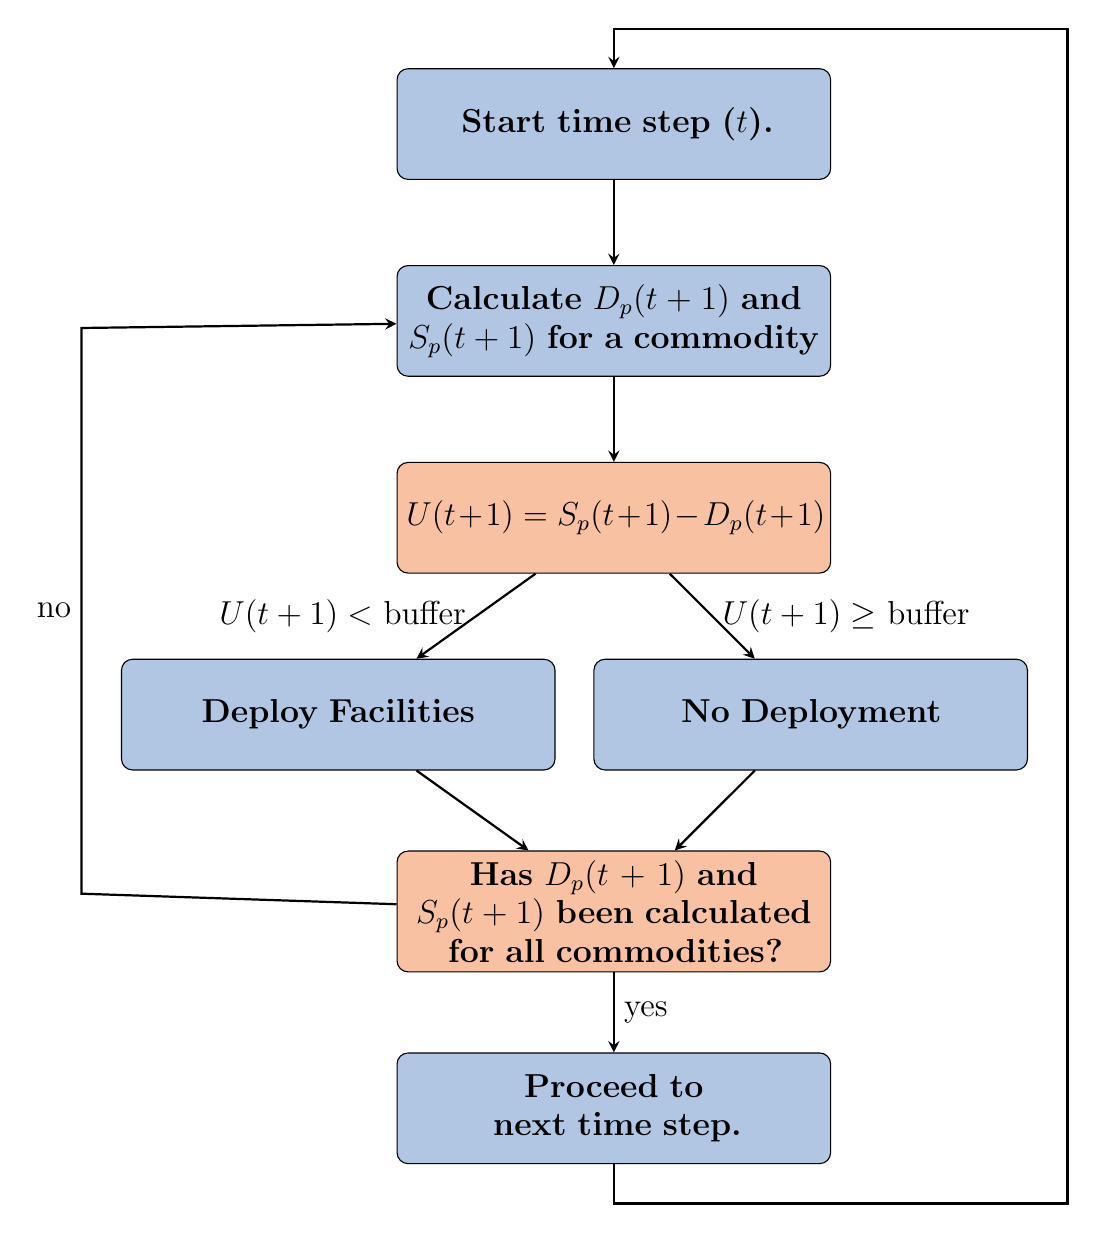
\begin{tikzpicture}[node distance=2.5cm]
    \tikzstyle{every node}=[font=\large]
	\node (Start) [bblock] {\textbf{Start time step ($t$).}};
	\node (Predict) [bblock, below of=Start] {\textbf{Calculate $D_p(t+1)$ and $S_p(t+1)$ for a commodity}};
	\node (IsThere) [oblock, below of=Predict]{\textbf{$U(t+1) = S_p(t+1)-D_p(t+1)$}};
	\node (Deploy) [bblock, below of=IsThere, xshift = -3.5cm]{\textbf{Deploy Facilities}};
    \node (NoDeploy) [bblock, right of=Deploy, xshift = 3.5cm]{\textbf{No Deployment} };
    \node (All) [oblock, below of=Deploy, xshift = 3.5cm] {\textbf{Has $D_p(t+1)$ and \\ $S_p(t+1)$ been calculated for all commodities?}};
    \node (End) [bblock, below of=All] {\textbf{Proceed to next time step.}};
	
	\draw [arrow] (Start) -- (Predict); 
	\draw [arrow] (Predict) -- (IsThere);
    \draw [arrow] (IsThere) -- node[anchor=east] {$U(t+1) <$ buffer} (Deploy);
    \draw [arrow] (IsThere) -- node[anchor=west] {$U(t+1) \geq$ buffer} (NoDeploy);
    \draw [arrow] (Deploy) -- (All);
    \draw [arrow] (NoDeploy) -- (All);
    \draw [arrow] (All) -- node[anchor=west] {yes} (End);
    \draw [arrow] (All) -- ([shift={(-4cm,1cm)}]All.south west)-- node[anchor=east] {no} ([shift={(-4cm,-0.8cm)}]Predict.north west)--(Predict);
    \draw [arrow] (End) |-([shift={(3cm,-0.5cm)}]End.south east)-- ([shift={(3cm,0.5cm)}]Start.north east)-|(Start);
	\end{tikzpicture}
	}
    \caption{\deploy logic flow at every time step in \Cyclus \cite{chee_demonstration_2019}.}
    \label{fig:flow}
\end{figure}

\deploy aims to minimize the undersupply of power:
\begin{align}
	\label{eq:pow}
	obj &= min \sum_{t=1}^{t_{f}} |D_{t,p}-S_{t,p}|.
	\intertext{where:}
	D &= \mbox{Demand} \nonumber\\
	S &= \mbox{Supply} \nonumber\\
	p &= \mbox{power} \nonumber \\
	t_f &= \mbox{Number of time steps} \nonumber \\
	M &= \mbox{Number of commmodities} \nonumber
\end{align} 
The sub-objectives are to minimize the number of time 
steps of undersupply or under-capacity of any 
commodity: 
\begin{align}
	\label{eq:sub1}
	obj = min \sum_{i=1}^{M}\sum_{t=1}^{t_f} |D_{t,i}-S_{t,i}|,
\end{align}
and to minimize excessive oversupply of all commodities: 
\begin{align}
	\label{eq:sub2}
	obj &= min \sum_{i=1}^{M}\sum_{t=1}^{t_f} |S_{t,i}-D_{t,i}|.
\end{align} 
Minimizing excessive oversupply 
reflects reality in which utilities avoid 
undersupply of power on the grid by ensuring power 
plants are never short of fuel while avoiding expensive oversupply.
Nuclear fuel cycle simulators often face power undersupplies 
due to lack of viable fuel, despite having sufficient installed 
reactor capacity.  
Using \deploy to automate the deployment of supporting 
facilities prevents this. 

\subsection{Structure}
%Description of front end and back end of fuel cycle 
%Demand Driven vs. Supply Driven 
In \deploy, two distinct institutions control 
front-end and back-end fuel cycle facilities: 
\texttt{DemandDrivenDeploymentInst} and 
\texttt{SupplyDrivenDeploymentInst}, respectively. 
The reason for this distinction is that front-end facilities 
meet the demand for commodities they produce, whereas back-end 
facilities meet supply for the commodities they demand. 
For example, when a reactor facility 
demands fuel, \texttt{DemandDrivenDeploymentInst}
deploys fuel fabrication facilities to create fuel
supply. 
For back-end facilities, the reactor generates spent fuel, and 
\texttt{SupplyDrivenDeploymentInst} deploys 
waste storage facilities to create capacity to store the spent fuel. 
Figure \ref{fig:insts} depicts a simple once-through fuel cycle 
and the \texttt{Institution} type governing each 
facility's deployment.  

\begin{figure}[]
	\centering
	\resizebox{\textwidth}{!}{
	\trimbox{0cm -.5cm 0cm 0cm}{ 
\begin{tikzpicture}[node distance=2.8cm,auto,>=latex']
	\tikzstyle{every node}=[font=\scriptsize]
    \node [bbslock] (a) {\textbf{Source}};
    \node [bbslock] (b) [right of=a] {\textbf{Enrichment \\ Facility}};
	\node [bbslock] (c) [right of=b] {\textbf{Reactor}};
	\node [obslock] (d) [right of=c] {\textbf{Cooling \\ Pool}};
	\node [obslock] (e) [right of=d] {\textbf{Sink}};
    \path[->] (a) edge node {\shortstack{Natl \\ U}} (b);
	\draw[->] (b) edge node {Fuel} (c) ;
	\draw[->] (c) edge node {\shortstack{Used \\ Fuel}} (d) ;
	\draw[->] (d) edge node {\shortstack{Cooled \\ Used \\ Fuel}} (e) ;
\end{tikzpicture}
	}}

\resizebox{0.5\textwidth}{!}{
    \fbox{\begin{tabular}{ll}
        \textcolor{illiniblue}{$\blacksquare$} & Deployed by \texttt{DemandDrivenDeploymentInst}\\
        \textcolor{illiniorange}{$\blacksquare$} & Deployed by \texttt{SupplyDrivenDeploymentInst} 
		\end{tabular}}}
		\caption{Simple once-through fuel cycle depicting which facilities are deployed by 
		\texttt{DemandDrivenDeploymentInst} and \texttt{SupplyDrivenDeploymentInst}.}
\label{fig:insts}
\end{figure}

\subsubsection{Deployment Driving Method}
The user may deploy facilities based on the difference 
between predicted demand and predicted supply, \textit{or}
predicted demand and installed capacity. 
Using installed capacity instead of predicted supply
has two advantages. 
First, to prevent over-deployment of facilities with an
intermittent supply such as reactors that require refueling. 
If predicted supply is selected instead of installed capacity, 
\deploy will deploy surplus reactors during refueling downtimes to 
meet the temporary power undersupply.
Second, to prevent infinite deployment of a facility that demands 
a commodity no longer available in the simulation. 
For example, a reprocessing plant that fabricates Sodium-Cooled Fast Reactor 
(SFR) fuel might demand Pu after depletion of the existing Pu inventory and 
decommissioning of the LWR reactors that produce it, resulting in 
infinite deployment of reprocessing facilities in a futile attempt 
to produce SFR fuel. 

\subsection{Input Variables}
Table \ref{tab:inputs} lists and gives examples of the input 
variables \deploy accepts. 
The user must do the following: 
define the facilities in the simulation, their respective 
capacities, the demand driving commodity,
its demand equation, the deployment driving method, 
and prediction method. 
The user also has the option to define supply/capacity buffers 
for individual commodities, facility preferences, and facility 
fleet shares.  
The subsequent sections describes 
the buffers, facility preferences, and prediction methods. 


\begin{table}[]
	\centering
    \caption{\deploy's required and optional input parameters with examples.}
    \label{tab:inputs}
        \footnotesize
        \begin{tabular}{l|ll}
        \hline
            & \textbf{Input Parameter}                                                           & \textbf{Examples}                                                                                                          \\ \hline
            \multirow{5}{*}{\textbf{Required}} & Demand driving commodity                                                           & Power                                                                                                                      \\ \cline{2-3} 
                                                      & Demand equation                                                                    & P(t) = 10000, sin(t), 10000*t                                                                                                                 \\ \cline{2-3} 
                                                      & Facilities it controls                                                             & Fuel Fab, LWR reactor, Sink, etc.                                                                                                      \\ \cline{2-3} 
                                                      & Capacities of the facilities                                                       & 3000 kg, 1000 MW, 50000 kg                                                                                                     \\ \cline{2-3} 
                                                      & Prediction method                                                                  & \begin{tabular}[c]{@{}l@{}}Power: fast fourier transform\\ Fuel: moving average\\ Spent fuel: moving average\end{tabular} \\ \cline{2-3} 
                                                      & Deployment driven by & Installed Capacity                                                                                                                    \\ \hline
            \multirow{4}{*}{\textbf{Optional}} & Supply/Capacity Buffer type                                                                        & Absolute                                                                                                                  \\ \cline{2-3} 
                                                      & Supply/Capacity Buffer size                                                                        & \begin{tabular}[c]{@{}l@{}}Power: 3000 MW\\ Fuel: 0 kg \\ Spent fuel: 0 kg\end{tabular}                                   \\ \cline{2-3} 
                                                      & Facility preferences                                                               & \begin{tabular}[c]{@{}l@{}}LWR reactor = 100-t\\ SFR reactor = t-99 \end{tabular}          \\ \cline{2-3} 
                                                      & Fleet share percentage                                                            & \begin{tabular}[c]{@{}l@{}}MOX LWR = 85\%\\ SFR = 15\% \end{tabular}          \\ \hline
                    \end{tabular}
\end{table}
\subsubsection{Supply/Capacity Buffer}
In \texttt{DemandDrivenDeploymentInst}, the user has the option to specify a 
supply buffer for each commodity; \deploy accounts for the buffer when 
calculating predicted demand and deploys facilities accordingly.
In \texttt{SupplyDrivenDeployment}

\noindent 
\texttt{Inst},
the user has the option to specify a capacity buffer for specific 
commodities; d3ploy accounts for the buffer when calculating predicted 
supply and deploys facilities accordingly. 
The buffer is defined as a percentage (equation \ref{eq:perc}) 
or absolute value (equation \ref{eq:abs}). 

\begin{align}
    \label{eq:perc}
	S_{pwb} &= S_{p}(1+d)\\
	\label{eq:abs}
	S_{pwb} &= S_{p}+b \\
	\intertext{where:}
	S_{pwb} &= \mbox{predicted supply/capacity with buffer} \nonumber\\
	S_p &= \mbox{predicted supply/capacity} \nonumber\\
	d &= \mbox{percentage value in decimal form} \nonumber\\
    b &= \mbox{absolute value of the buffer} \nonumber
\end{align}
For example, the user sets the power commodity's absolute supply buffer 
to be 2000 MW and predicted demand is 10000 MW, \deploy deploys reactor 
facilities to meet the predicted demand and supply buffer, resulting 
in a power supply of: 
\begin{align*}
	S_{pwb} &= S_{p}+a \\
	S_{pwb} &= 10000 \mbox{MW}+2000 \mbox{MW} \\
	&= 12000\mbox{MW}
\end{align*}
Using the buffer capability and  
installed capacity to drive facility deployment in a transition 
scenario simulation will effectively minimize undersupply of a 
commodity while avoiding excessive oversupply. 
This is demonstrated in Section \ref{sec:demo}. 

\subsection{Facility Preference and Fleet Share}

The user has the option to give time-dependent preference 
equations to facilities' that supply the same commodity. 
If there are two reactor types, \glspl{LWR} and \glspl{SFR}, in a simulation, 
the user can make use of time-dependent 
preferences to make the simulation deploy LWRs at earlier times 
in the simulation, and deploy SFRs at later times in the 
simulation when there is a power demand. 
In table \ref{tab:inputs}, 
the LWR has a preference of $100-t$, and the 
SFR has a preference of $t-99$. 
$t$ refers to the month timestep. 
At time step 1, LWR preference becomes 99, while SFR preference becomes -98; 
therefore a LWR is deployed if there is a commodity shortage. 
At time step 100, LWR preference becomes 0, while SFR preference becomes 1; 
therefore a SFR is deployed if there is a commodity shortage. 
Thus, the transition occurs at the $100^{th}$ time step.

The user also has the option to specify percentage-share for facilities 
that provide the same commodity. 
For example, if there are two reactor types, \gls{MOX} LWRs and SFRs, in a simulation,
the user can make use of percentage-share specifications to determine the 
percentage of power supplied by each reactor.   
When MOX LWR has a share of $s\%$ and 
\gls{SFR} has a share of $(100-s)\%$, 
MOX LWR deployment constrains to $s\%$ of total power demand 
and SFR deployment constrains to $(100-s)\%$ of total power demand.  

The year the transition begins is selected by customizing facility 
preferences to begin preference for advanced reactors at a certain year,
and the sharing capability determines the percentage 
share of each type of reactor to transition to. 
Therefore, when \deploy predicts an undersupply of a commodity 
it deploys facilities in order of preference, starting at 
the highest and moving down if the facility percentage share 
is already met. 
If a facility type does not have any preferences, \deploy 
deploys available facilities to minimize the number of deployed 
facilities and oversupply of the commodity.


Figure \ref{fig:deployflow} shows the logical flow of how \deploy 
selects which facility to deploy when there are multiple facilities 
offering the same commodity. 

\begin{figure}[]
	\centering
	\resizebox{\textwidth} {0.8\height}{
    \begin{tikzpicture}[node distance=2.5cm]
    \tikzstyle{every node}=[font=\large]
	\node (pref)[olblock]{\textbf{Are there facility preferences?}};
	\node (fs1) [oblock, below of=pref, xshift = -3.5cm]{\textbf{Are there fleet share constraints?}};
	\node (fs2) [oblock, right of=fs1, xshift = 3.5cm]{\textbf{Are there fleet share constraints?} };
	\node (fs2yes) [bbmlock, below of=fs2, xshift = -2cm] {\textbf{Deploy facilities to meet fleet share $\%$}};
	\node (fs2no) [bbmlock, right of=fs2yes, xshift = 2cm, yshift=-1.07cm] {\textbf{Deploy facilities to minimize total no. of facilities and minimize oversupply.}};
	\node (fs1yes) [bbmmlock, below of=fs1, xshift = -2cm, yshift=-3cm] {\textbf{Deploy facilities in preference order to meet their fleet share \%}};
	\node (fs1no) [bbmlock, right of=fs1yes, xshift = 2cm] {\textbf{Deploy facility with highest preference}};
    \draw [arrow] (pref) -- node[anchor=east] {yes} (fs1);
	\draw [arrow] (pref) -- node[anchor=west] {no} (fs2);
	\draw [arrow] (fs2) -- node[anchor=east] {yes} (fs2yes);
	\draw [arrow] (fs2) -- node[anchor=west] {no} (fs2no);
	\draw [arrow] (fs1) -- node[anchor=east] {yes} (fs1yes);
	\draw [arrow] (fs1) -- node[anchor=west] {no} (fs1no);
	\end{tikzpicture}
	}
    \caption{Logical flow of how \deploy 
	selects which facility to deploy when there are multiple facilities 
	offering the same commodity.}
	\label{fig:deployflow}
\end{figure}

\subsection{Prediction Methods}
\deploy records supply and demand values at each time step for all 
commodities to provide time-series data for \deploy's time series 
forecasting methods to predict future supply and demand for each 
commodity.  
The time series forecasting methods investigated include non-optimizing, 
deterministic-optimizing, and stochastic-optimizing methods. 
Non-optimizing methods are techniques that harness 
simple moving average and autoregression concepts which use 
historical data to infer future supply and demand values. 
Deterministic-optimizing and stochastic-optimizing 
methods are techniques 
that use an assortment of more sophisticated time series forecasting 
concepts to predict future supply and demand values. 
Deterministic-optimizing methods give deterministic solutions,
while stochastic-optimizing methods give stochastic solutions. 

Depending on the scenario in question, each forecasting method 
offers distinct benefits and disadvantages.
The various methods are compared for each type of simulation 
to determine the most effective prediction method for 
a given scenario. 
The following sections describe the prediction methods. 

\subsubsection{Non-Optimizing Methods}
Non-optimizing methods include: Moving Average (\texttt{MA}), 
Autoregressive Moving Average (\texttt{ARMA}), and 
Autoregressive Heteroskedasticity (\texttt{ARCH}). 
The \texttt{MA} method calculates the average of 
a user-defined number of previous entries in a commodity's 
time series and returns it as the predicted value 
(equation \ref{eq:ma}).

\begin{align}
	\label{eq:ma}
	Predicted\ Value &= \frac{V_1+V_2+...+V_n}{n}
	\intertext{where:}
	V &= \mbox{Time series value} \nonumber\\
	n &= \mbox{length of timeseries} \nonumber\\
\end{align}

The \texttt{ARMA} method combines moving average and
autoregressive models (equation \ref{eq:arma}).
The first term is a constant, second term is 
white noise, the third term is the autoregressive
model, and the fourth term is the moving average
model.
The \texttt{ARMA} method is more accurate than the 
\texttt{MA} method 
because of the inclusion of the autoregressive term. 

\begin{align}
	\label{eq:arma}
	X_t &= c + \epsilon_t + 
	\sum_{i=1}^p\varphi_i X_{t-i} +	
	\sum_{i=1}^q\theta_i\epsilon_{t-i}
	\intertext{where:}
	c &= \mbox{constant} \nonumber\\
	\varphi &= \mbox{parameters} \nonumber\\
	\epsilon_t &= \mbox{white noise} \nonumber\\
	p &= \mbox{equation order} \nonumber \\
\end{align}

The \texttt{ARCH} method modifies the original moving 
average term (described in equation \ref{eq:arma}). 
This modification makes the \texttt{ARCH} method 
better than the \texttt{ARMA} method for volatile 
time-series data \cite{flanagan_methods_2019}. 
The StatsModels \cite{github_community_statsmodels:_2019}
Python package is used to implement \texttt{ARMA} and 
\texttt{ARCH} methods in \deploy. 

\subsubsection{Deterministic-Optimizing Methods}
Deterministic methods include
Fast Fourier Transform (\texttt{FFT}), 
Polynomial Fit (\texttt{POLY}), 
Exponential Smoothing (\texttt{EXP-SMOOTHING}), 
and Triple Exponential Smoothing (\texttt{HOLT-WINTERS}). 
The \texttt{FFT} method computes the discrete Fourier transform 
of the time series to predict future demand and supply 
values (equation \ref{eq:fft}).
This method is implemented in \deploy using the 
SciPy \cite{jones_scipy:_2016} Python package. 

\begin{align}
	\label{eq:fft}
	X_k &= \sum_{n=0}^{N-1}x_n e^{-i2\pi kn/N}
	\intertext{where:}
	k &= 0, ..., N-1 \nonumber\\
	N &= \mbox{No. of data points} \nonumber
\end{align}

The \texttt{POLY} method models the time series data 
with a user-defined nth degree polynomial to determine 
future demand and supply values. 
This method was implemented in \deploy using the 
NumPy \cite{developers_numpy_2013} Python package. 
The \texttt{EXP-SMOOTHING} and \texttt{HOLT-WINTERS} 
methods use a weighted average 
of time-series data with exponentially decaying weights 
for older time series values \cite{hyndman_forecasting:_2018}
to create a model to determine future demand and supply values. 
The \texttt{EXP-SMOOTHING} method excels in 
modeling univariate time series data without trend or seasonality, 
whereas the \texttt{HOLT-WINTERS} method applies exponential 
smoothing three times, resulting in higher accuracy when 
modeling seasonal time series data. 
The StatsModels \cite{github_community_statsmodels:_2019}
Python package was used to implement both of these methods 
in \deploy. 

\subsection{Stochastic-Optimizing Methods}
There is one stochastic-optimizing method: step-wise 
seasonal method (\texttt{SW-SEASONAL}). 
The method was implemented in \deploy by the auto \gls{ARIMA} 
method in the pmdarima \cite{noauthor_pmdarima:_2019}
Python package. 
The \gls{ARIMA} model is a generalization of the \gls{ARMA}
model to make the model fit the time series data better. 


% Methodology: Overall objectives of d3ploy and how it works
% Structure (Demand/Supply Driven Inst)
% Input variables
% Deployment driving method (installedcap)
% Supply/Capacity Buffer 
% Prediction Methods
\FloatBarrier
\section{Results}
To demonstrate \deploy's capability conduct transition
scenario analysis effectively and meet the objectives described in section 
\ref{sec:obj}, this section 
(1) demonstrates \deploy's capability in a simple transition scenario, 
(2) compares the use of different \deploy prediction methods in EG01-EG23, EG01-EG24, 
EG01-EG29, and EG01-EG30 transition scenarios, and
(3) demonstrates successful \deploy setup of EG01-EG23, EG01-EG24, 
EG01-EG29, and EG01-EG30 transition scenarios. 
The input files and scripts to reproduce the results and plots in this
paper are found in \cite{noauthor_arfc/d3ploy:_2019} and 
\cite{chee_arfc/transition-scenarios_2019}. 

\subsection{Demonstration of \deploy's Capabilities}
\label{sec:demo}
We conducted a simple transition scenario simulation with
linearly increasing power demand
to demonstrate \deploy's capabilities and inform input parameter 
choices when setting up complex many-facility transition scenarios. 
This simulation is defined as \textit{simple} since 
it only includes
three facility types: \texttt{source}, \texttt{reactor}, and 
\texttt{sink}. 
The simulation begins with ten \texttt{reactor} facilities 
(\texttt{reactor1} to \texttt{reactor10}). 
These reactors have staggered cycle lengths and lifetimes to prevent 
simultaneous refueling and set up gradual decommissioning. 
\deploy is configured to deploy \texttt{new reactor} facilities
to meet the loss of power supply created by the decommissioning 
of the initial \texttt{reactor} facilities. 
Table \ref{tab:demonstrations} shows the \deploy input parameters 
for this simulation.  

    \begin{table}[]
        \caption{\deploy's input parameters for the simple transition 
        scenario with linearly increasing power demand.}
        \label{tab:demonstrations}
        \begin{tabular}{l|ll}
        \hline
                                  & \textbf{Input Parameters}          & \textbf{Simple Transition Scenario} \\ \hline
        \multirow{5}{*}{\textbf{Required}} & Demand driving commodity  & \multicolumn{1}{l}{Power}                            \\
                                  & Demand equation [MW]          &  $t<40 = 1000, t\geq 40 = 1000+250t$                                                    \\
                                  & Available facilities    &  \texttt{Source}, \texttt{Reactor}, \texttt{Sink}                                                    \\
                                  & Prediction method         &  \texttt{FFT}                                                    \\
                                  & Deployment driving method & \multicolumn{1}{l}{Installed Capacity}               \\ \hline
        \multirow{2}{*}{\textbf{Optional}} & Buffer type               & \multicolumn{1}{l}{Absolute}                         \\
                                  & Buffer size               &  Power: 2000MW, Fuel: 1000kg                                                    \\ \hline
        \end{tabular}%
        \end{table}

Figures \ref{fig:growingtransition-power}, \ref{fig:growingtransition-fuel},
and \ref{fig:growingtransition-spentfuel} demonstrate \deploy's capability 
to deploy reactors and supporting facilities to minimize undersupply 
when meeting linearly increasing power demand and subsequent secondary 
commodities demand. 
In Figure \ref{fig:growingtransition-power} there exists no time steps 
in which the supply of power falls under demand, meeting the main 
objective of \deploy. 
By using a combination of the \texttt{FFT} method for 
predicting demand and a power supply buffer of 2000MW 
(the capacity of 2 reactors), we minimized the number of 
undersupplied time steps for every commodity.

In figure \ref{fig:growingtransition-fuel},
a large-throughput source facility is initially
deployed to meet the large initial fuel demand for the commissioning 
of ten reactors. 
Deployment of a large-throughput source facility for the 
first few time steps ensures \deploy does not deploy supporting
facilities that become redundant at later times in  
the simulation.
This reflects reality in which reactor manufacturers accumulate
an appropriate amount of fuel inventory before starting 
up reactors. 

\begin{figure}[]
    \centering
    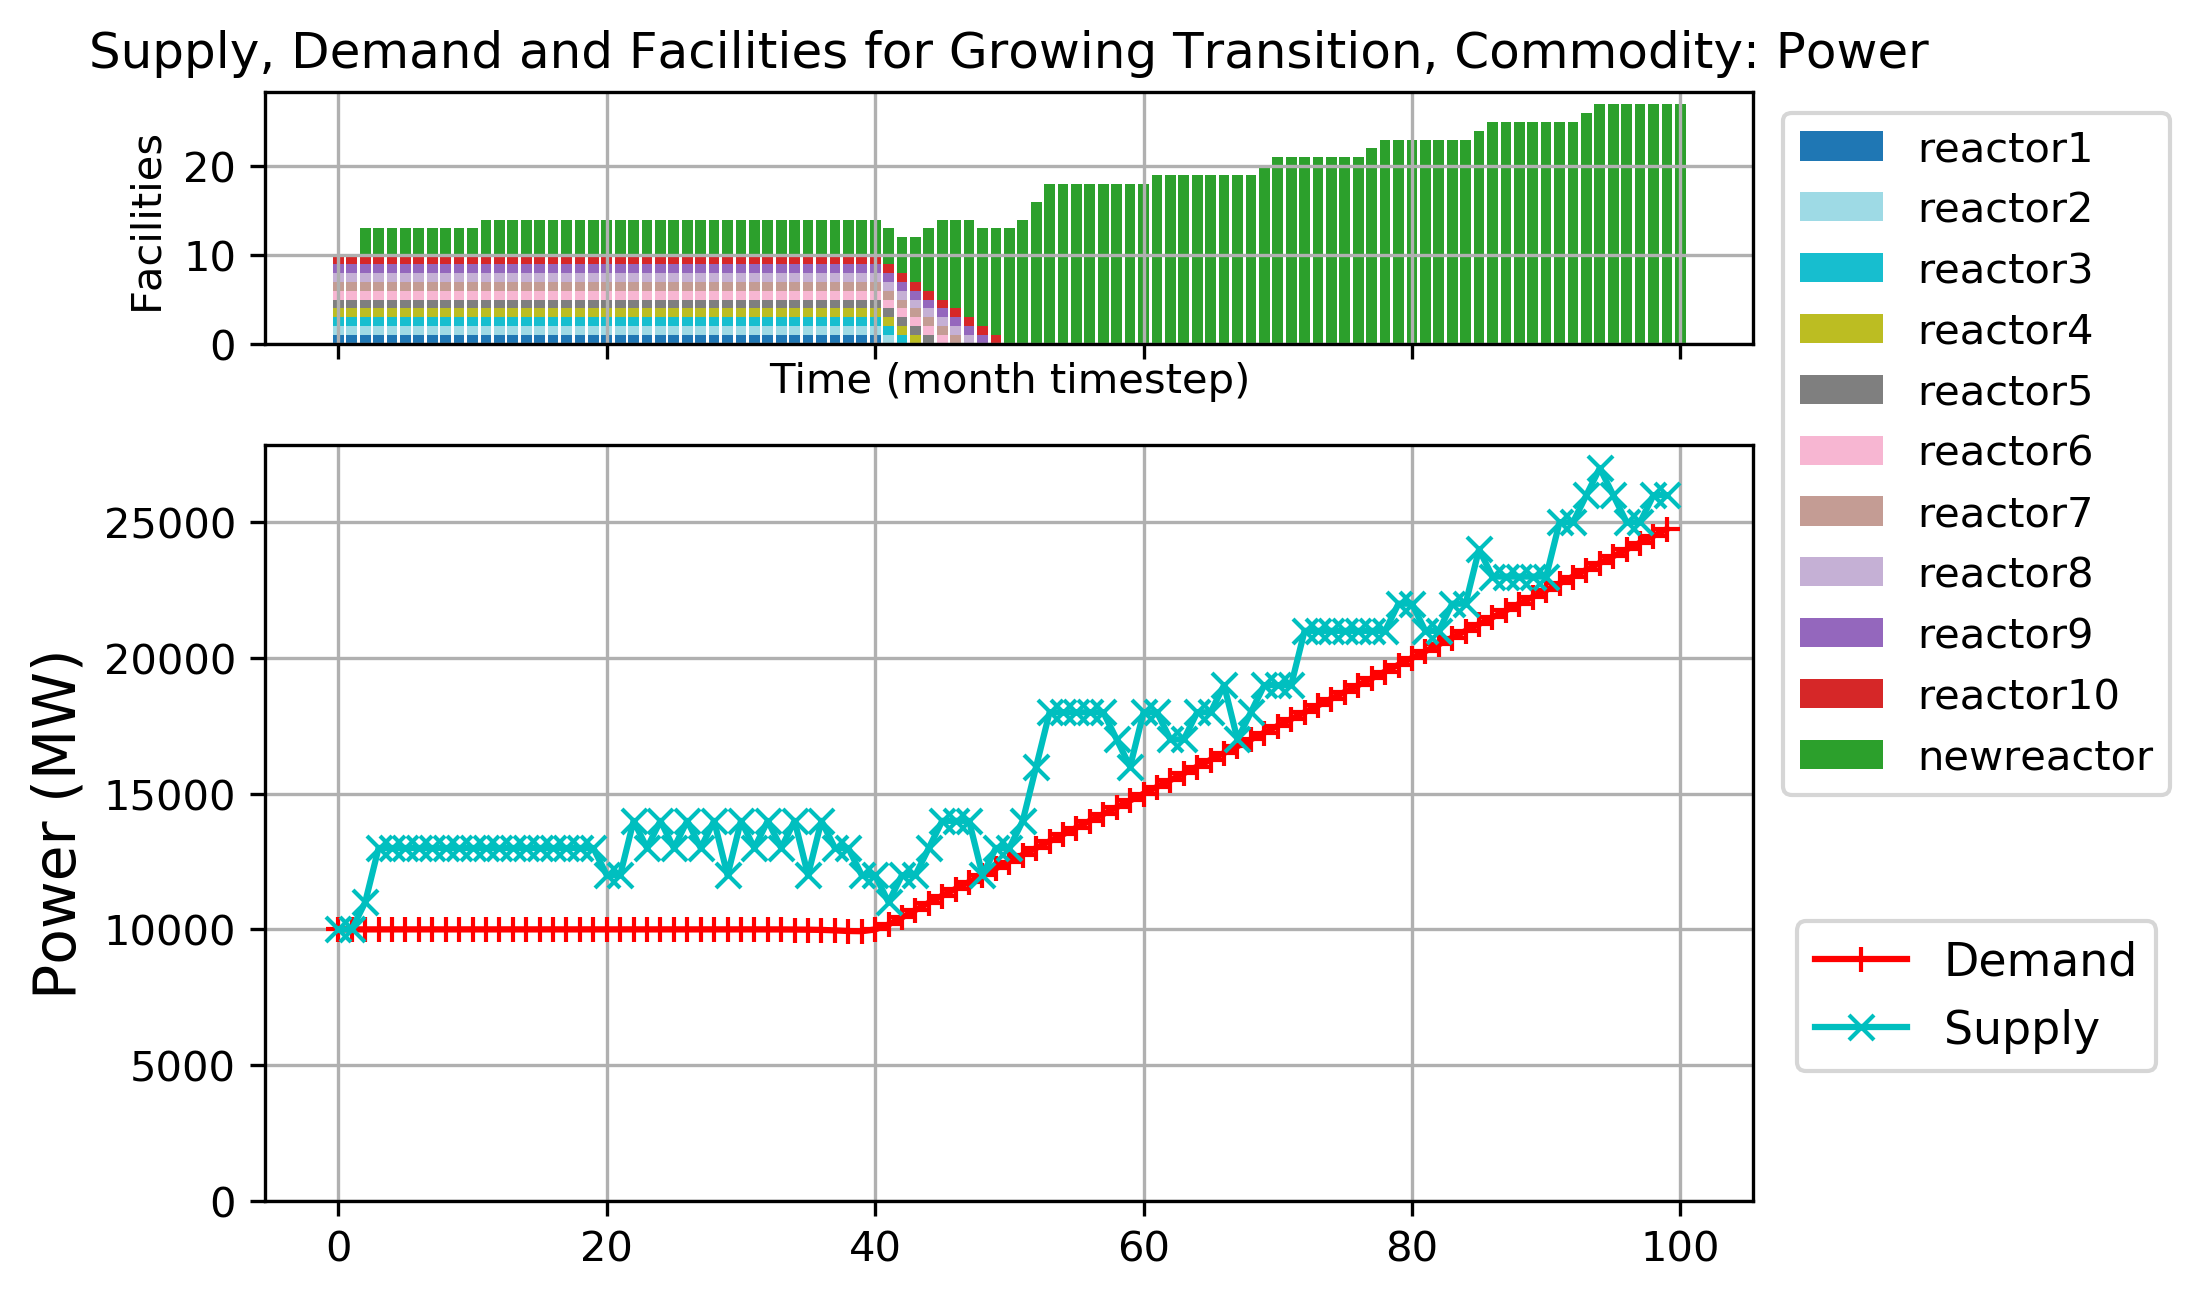
\includegraphics[width=\linewidth]{figures/growingtransition-power.png} 
        \caption{Power demand and supply, and reactor facility deployment plot for  
        a simple linearly increasing power demand transition scenario with 
        three facility types: \texttt{source}, \texttt{reactor}, and \texttt{sink}.
        The simulation begins with \texttt{reactor1} to \texttt{reactor10} and \deploy 
        deploys \texttt{newreactors} to meet increasing power demand. 
        Power undersupply was avoided entirely.}
        \label{fig:growingtransition-power}
\end{figure}

\begin{figure}[]
    \centering
    \begin{subfigure}[t]{1\textwidth}
        \centering
        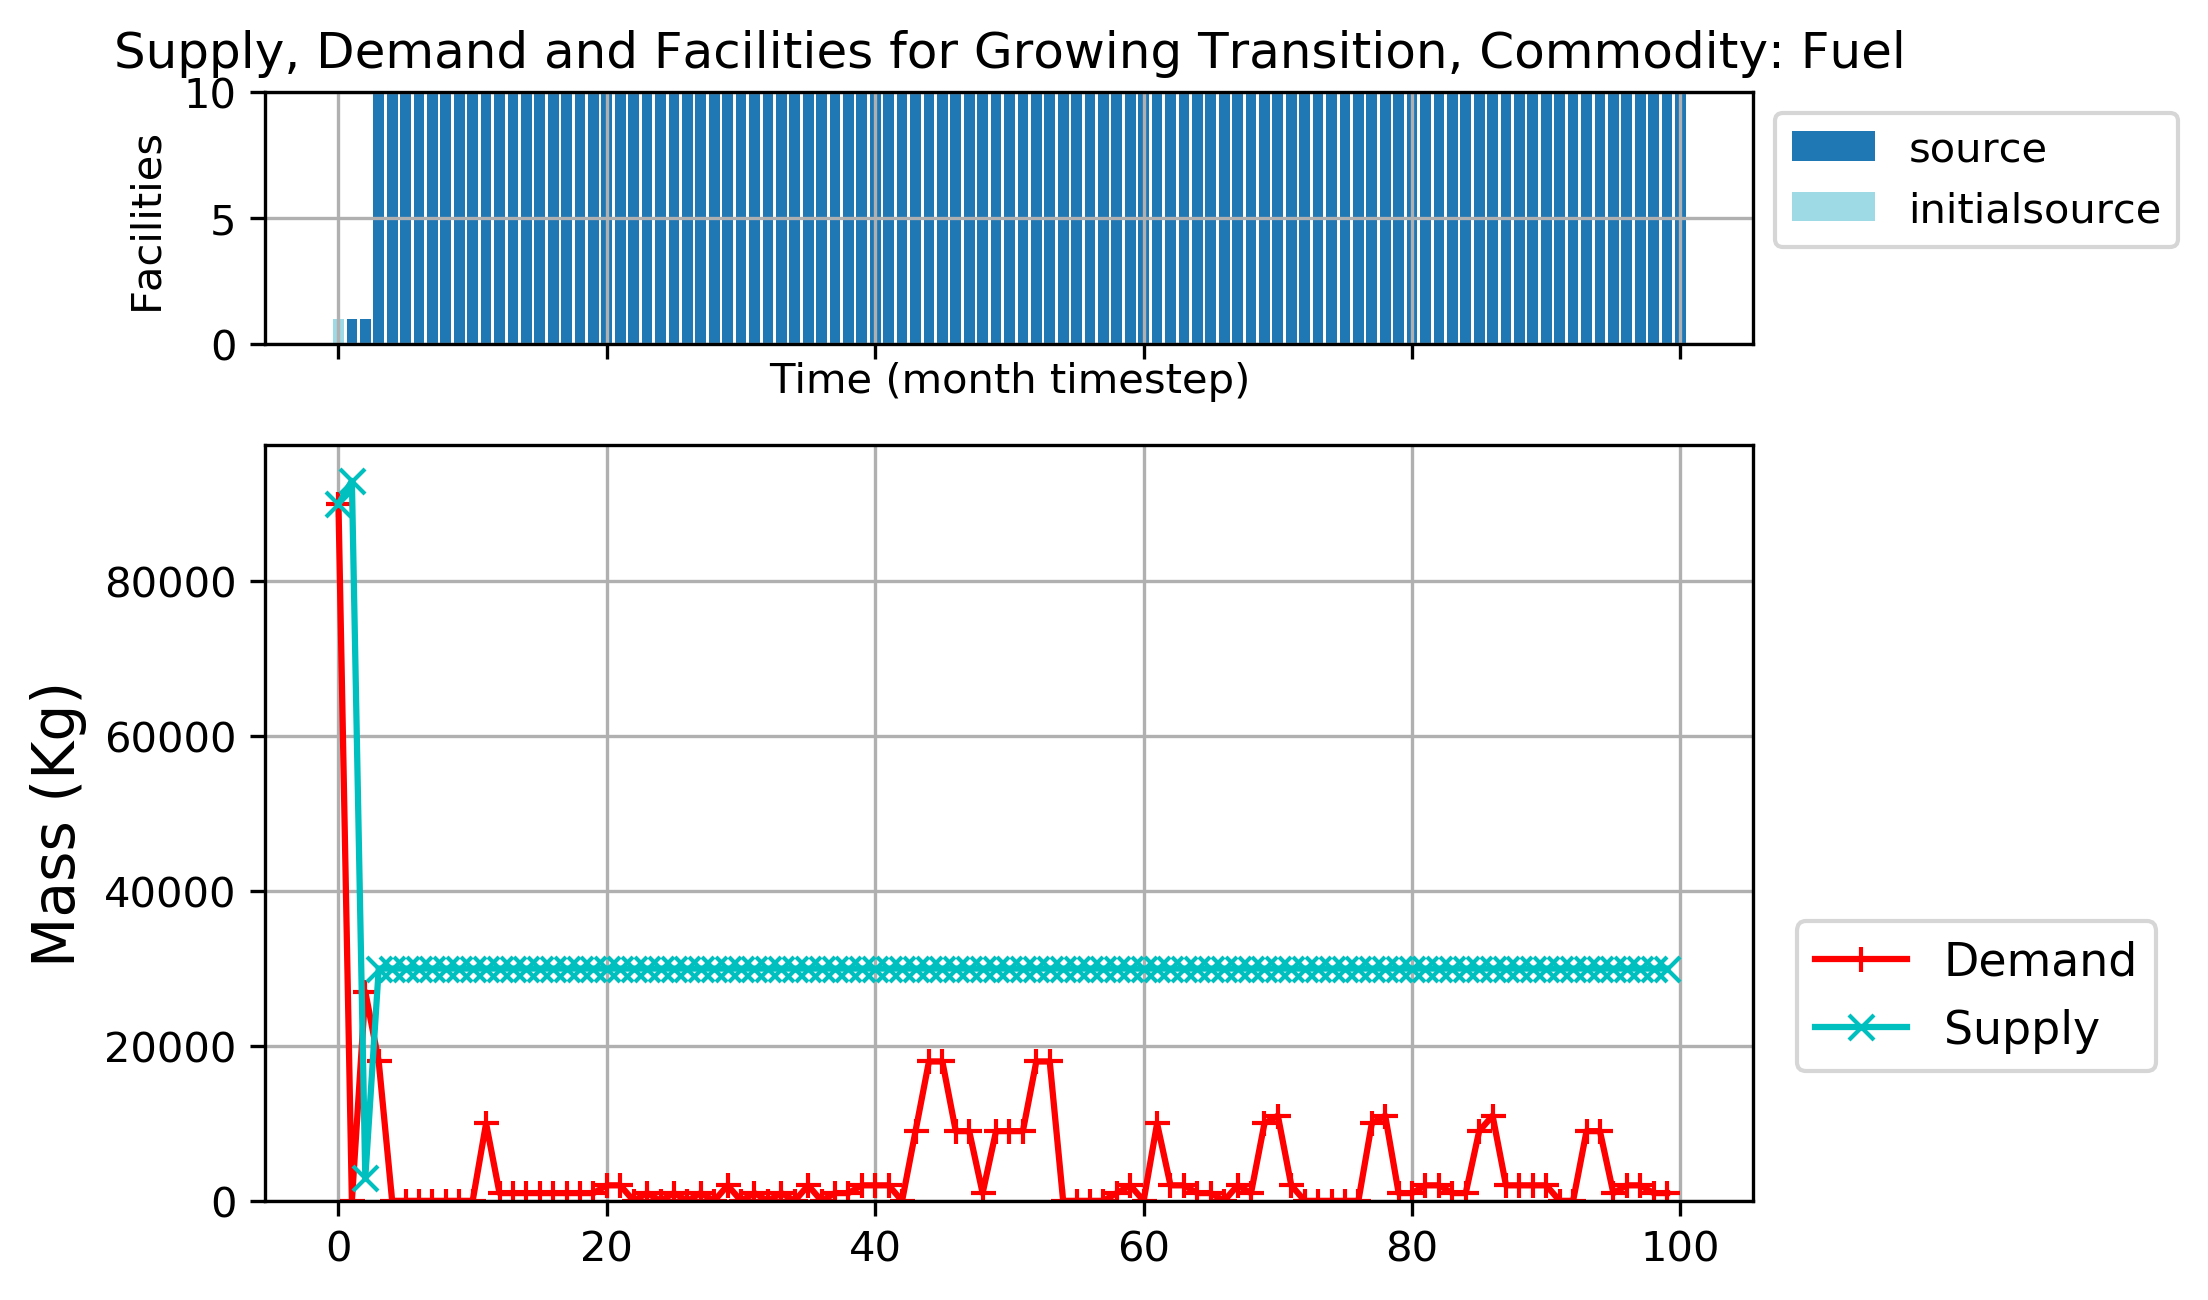
\includegraphics[width=\linewidth]{figures/growingtransition-fuel.png} 
        \caption{Fuel demand and supply, and source facility deployment plot.
        Fuel is demanded by reactors and supplied by source facilities.
        There is only one time step with undersupply of fuel.}
	    \label{fig:growingtransition-fuel}
    \end{subfigure}
    \begin{subfigure}[t]{1\textwidth}
        \centering
        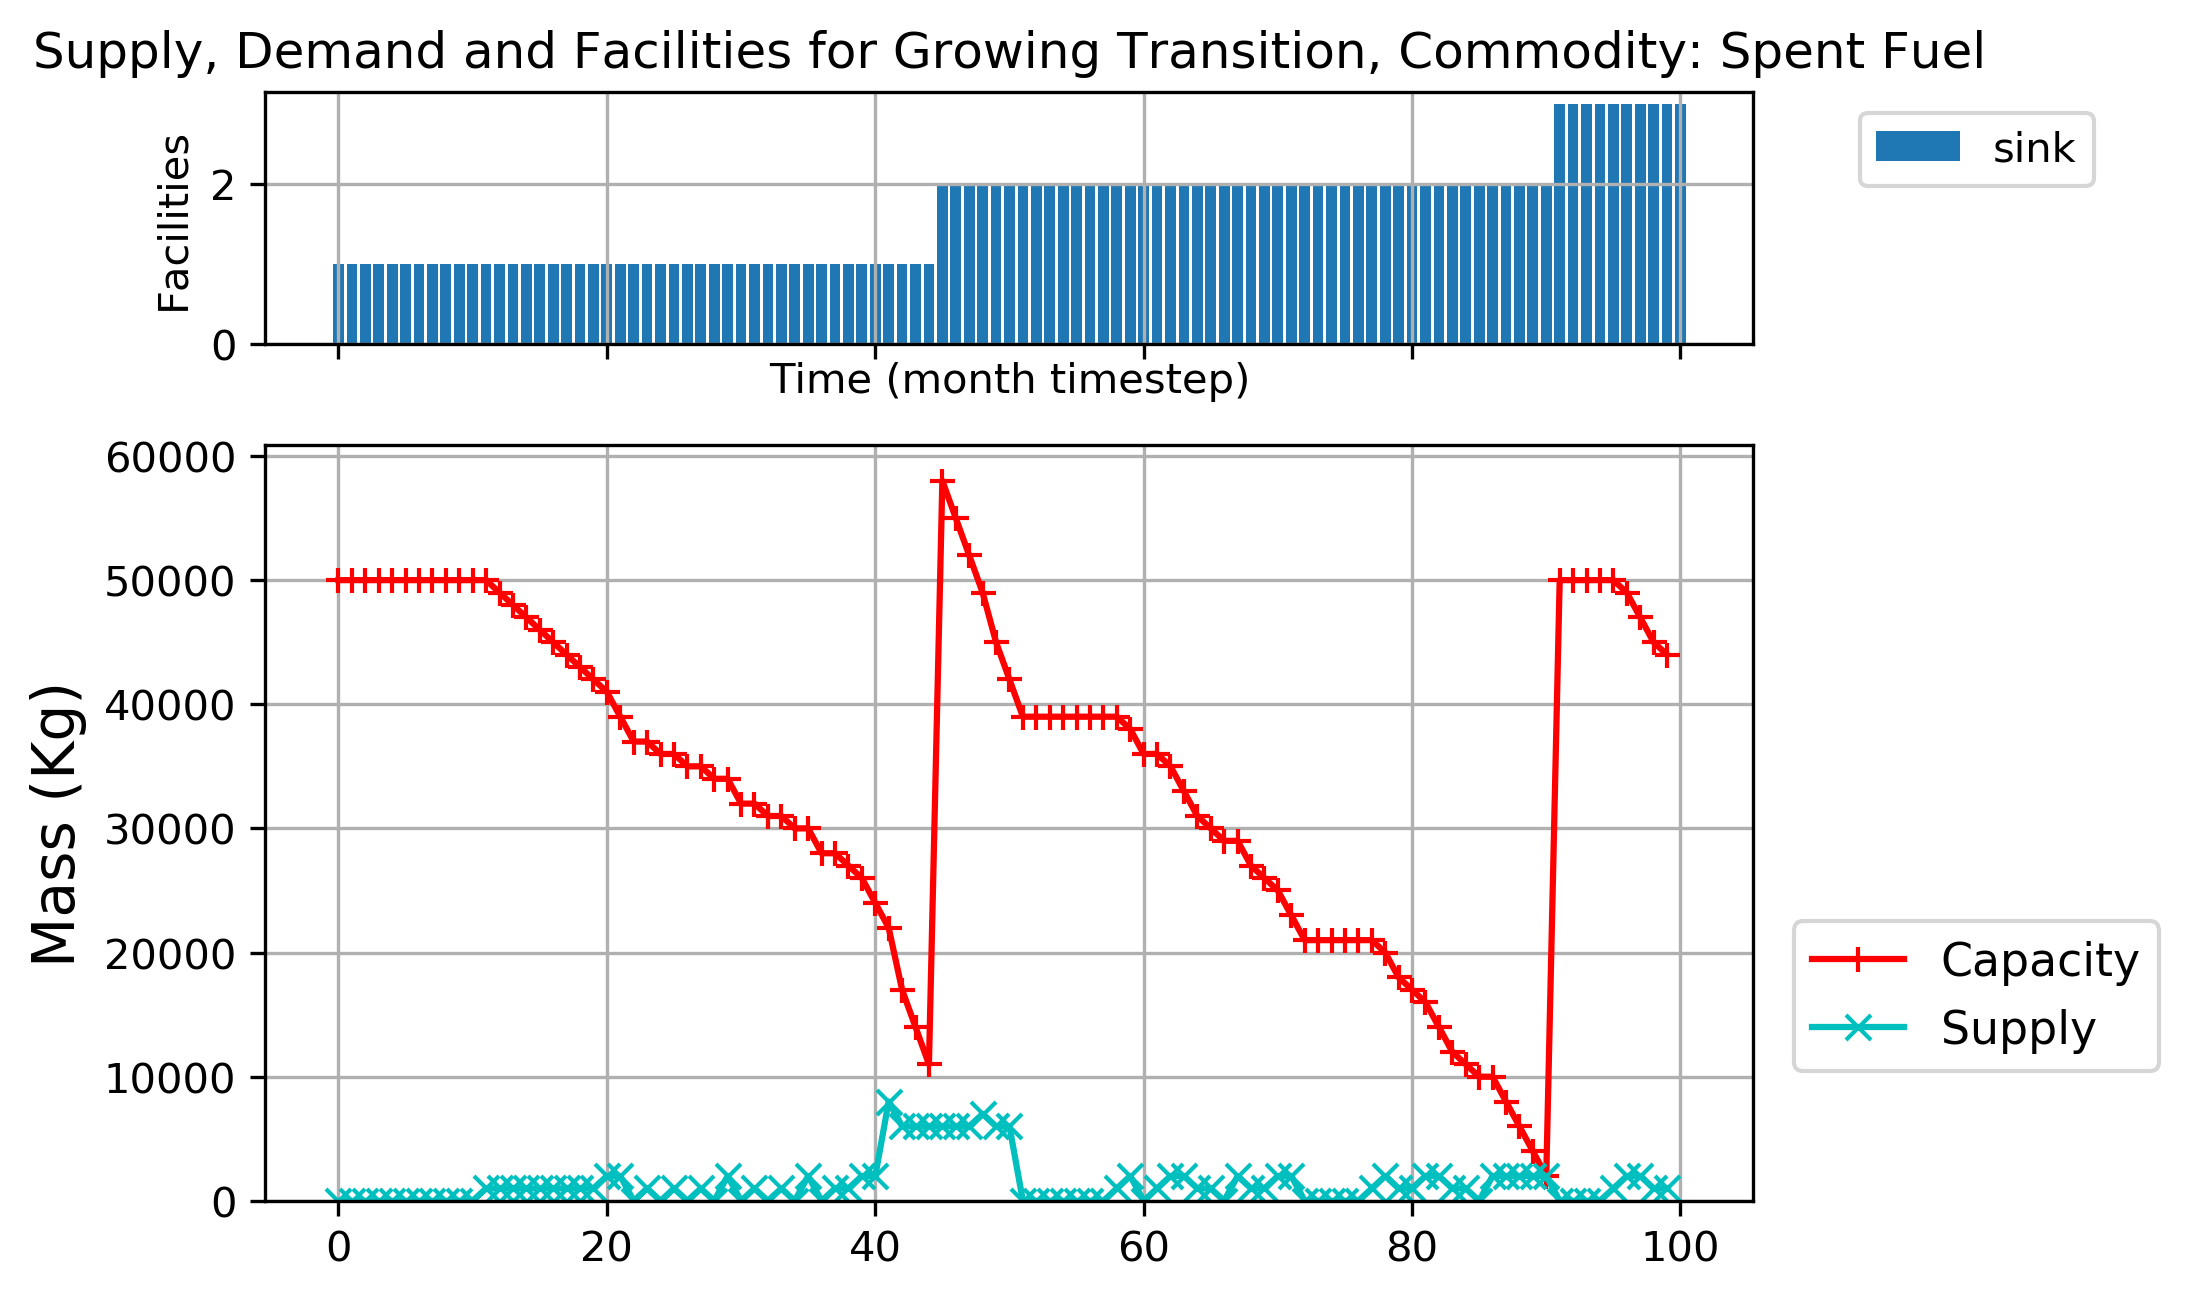
\includegraphics[width=\linewidth]{figures/growingtransition-spentfuel.png} 
        \caption{Spent fuel capacity and supply, and sink facility deployment plot.
            Spent fuel is supplied by reactors and the capacity to store them 
            is provided by sink facilities.
        There are no time steps with under-capacity of sink space.}
        \label{fig:growingtransition-spentfuel}
    \end{subfigure}
    \caption{Simple linearly increasing power demand transition scenario with 
    three facility types: \texttt{source}, \texttt{reactor}, and \texttt{sink}.}
\end{figure}

\subsection{Comparison of Prediction Methods}

EG01-EG23, EG01-EG24, EG01-EG29, and EG01-EG30 transition scenarios
are set up in \Cyclus using \deploy. 
EG01-23 and EG01-29 transition scenario simulations have a constant 
power demand, while EG01-24 and EG01-30 have a linearly increasing
power demand. 
We identified the most effective d3ploy prediction method 
for each scenario by comparing the results of using each 
prediction method in each scenario. 
Similar to the simple transition scenario, these transition scenario 
simulations begin with an initial fleet of \glspl{LWR} 
that start progressively decommissioning at the 80-year mark, 
after which \deploy deploys \glspl{SFR} and \gls{MOX} \glspl{LWR} to meet 
the power demand. 
Figure \ref{fig:eg2329}
shows the setup of facilities and mass flows for 
EG01-23 and EG01-29 in \Cyclus. 
In EG01-23 and EG01-29, recycled plutonium from LWR spent fuel 
produces  \gls{SFR} fuel. 
EG01-24 and EG01-30 are similar to EG01-23 and EG01-29, respectively, 
with the exception that all transuranic elements are recycled.

\begin{figure}[]
	\centering
	\begin{subfigure}[t]{\textwidth}
		\centering
		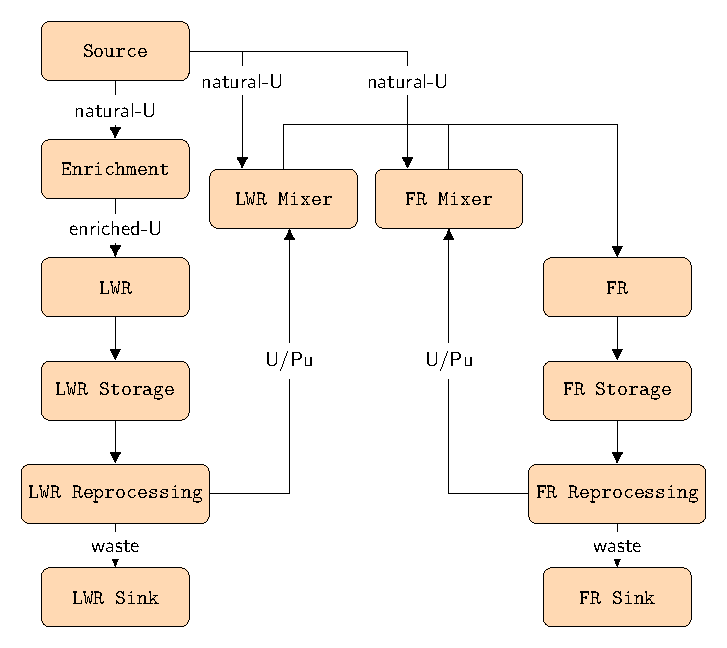
\includegraphics[width=0.8\linewidth]{23flow.pdf} 
		\caption{EG01-EG23.}
		\label{fig:23flow}
	\end{subfigure}
	\vspace{1cm}
	\begin{subfigure}[t]{\textwidth}
		\centering
		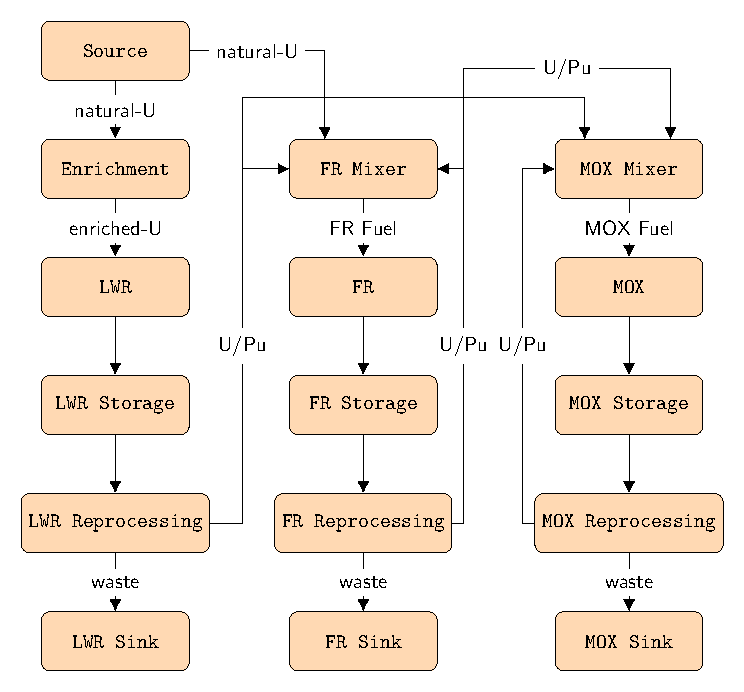
\includegraphics[width=0.8\linewidth]{29flow.pdf} 
		\caption{EG01-EG29.}
		\label{fig:29flow}
	\end{subfigure}
	\hfill
	\caption{Facility and mass flow of the transition scenarios EG01-EG23 and EG01-EG29 in \Cyclus.}
	\label{fig:eg2329}
\end{figure}

In Figure \ref{fig:eg23under}, each histogram represents 
the number of time steps with undersupply or 
under capacity for all commodities for each prediction method.  
Table \ref{tab:all-power} shows the number of time steps with power 
undersupply for constant power EG01-EG23 and EG01-29, 
linearly increasing power EG01-24 and EG01-30 transition scenarios. 
Figure \ref{fig:eg23under} demonstrates that the \texttt{POLY} method
perform the best for the EG01-23 transition scenario,
with the smallest bars on the plot, indicating that they have the 
fewest number of time steps with undersupply and under capacity
of commodities. 
We conducted a similar analysis for the constant power EG01-29 scenario,
and as seen in Table \ref{tab:all-power}, the \texttt{POLY} prediction method 
also performed best for minimizing undersupply of power.  

In Figure \ref{fig:eg24under}, each histogram represents 
the number of time steps with undersupply or 
under capacity for all commodities for each prediction method.  
Figure \ref{fig:eg24under} demonstrates that the \texttt{FFT} method 
perform the best for the EG01-24 transition scenario.
We conducted a similar analysis for the linearly increasing power 
EG01-30 scenario, and 
as seen in Table \ref{tab:all-power}, the \texttt{FFT} prediction method 
also performed best for minimizing undersupply of power. 

\begin{figure}[]
	\centering
	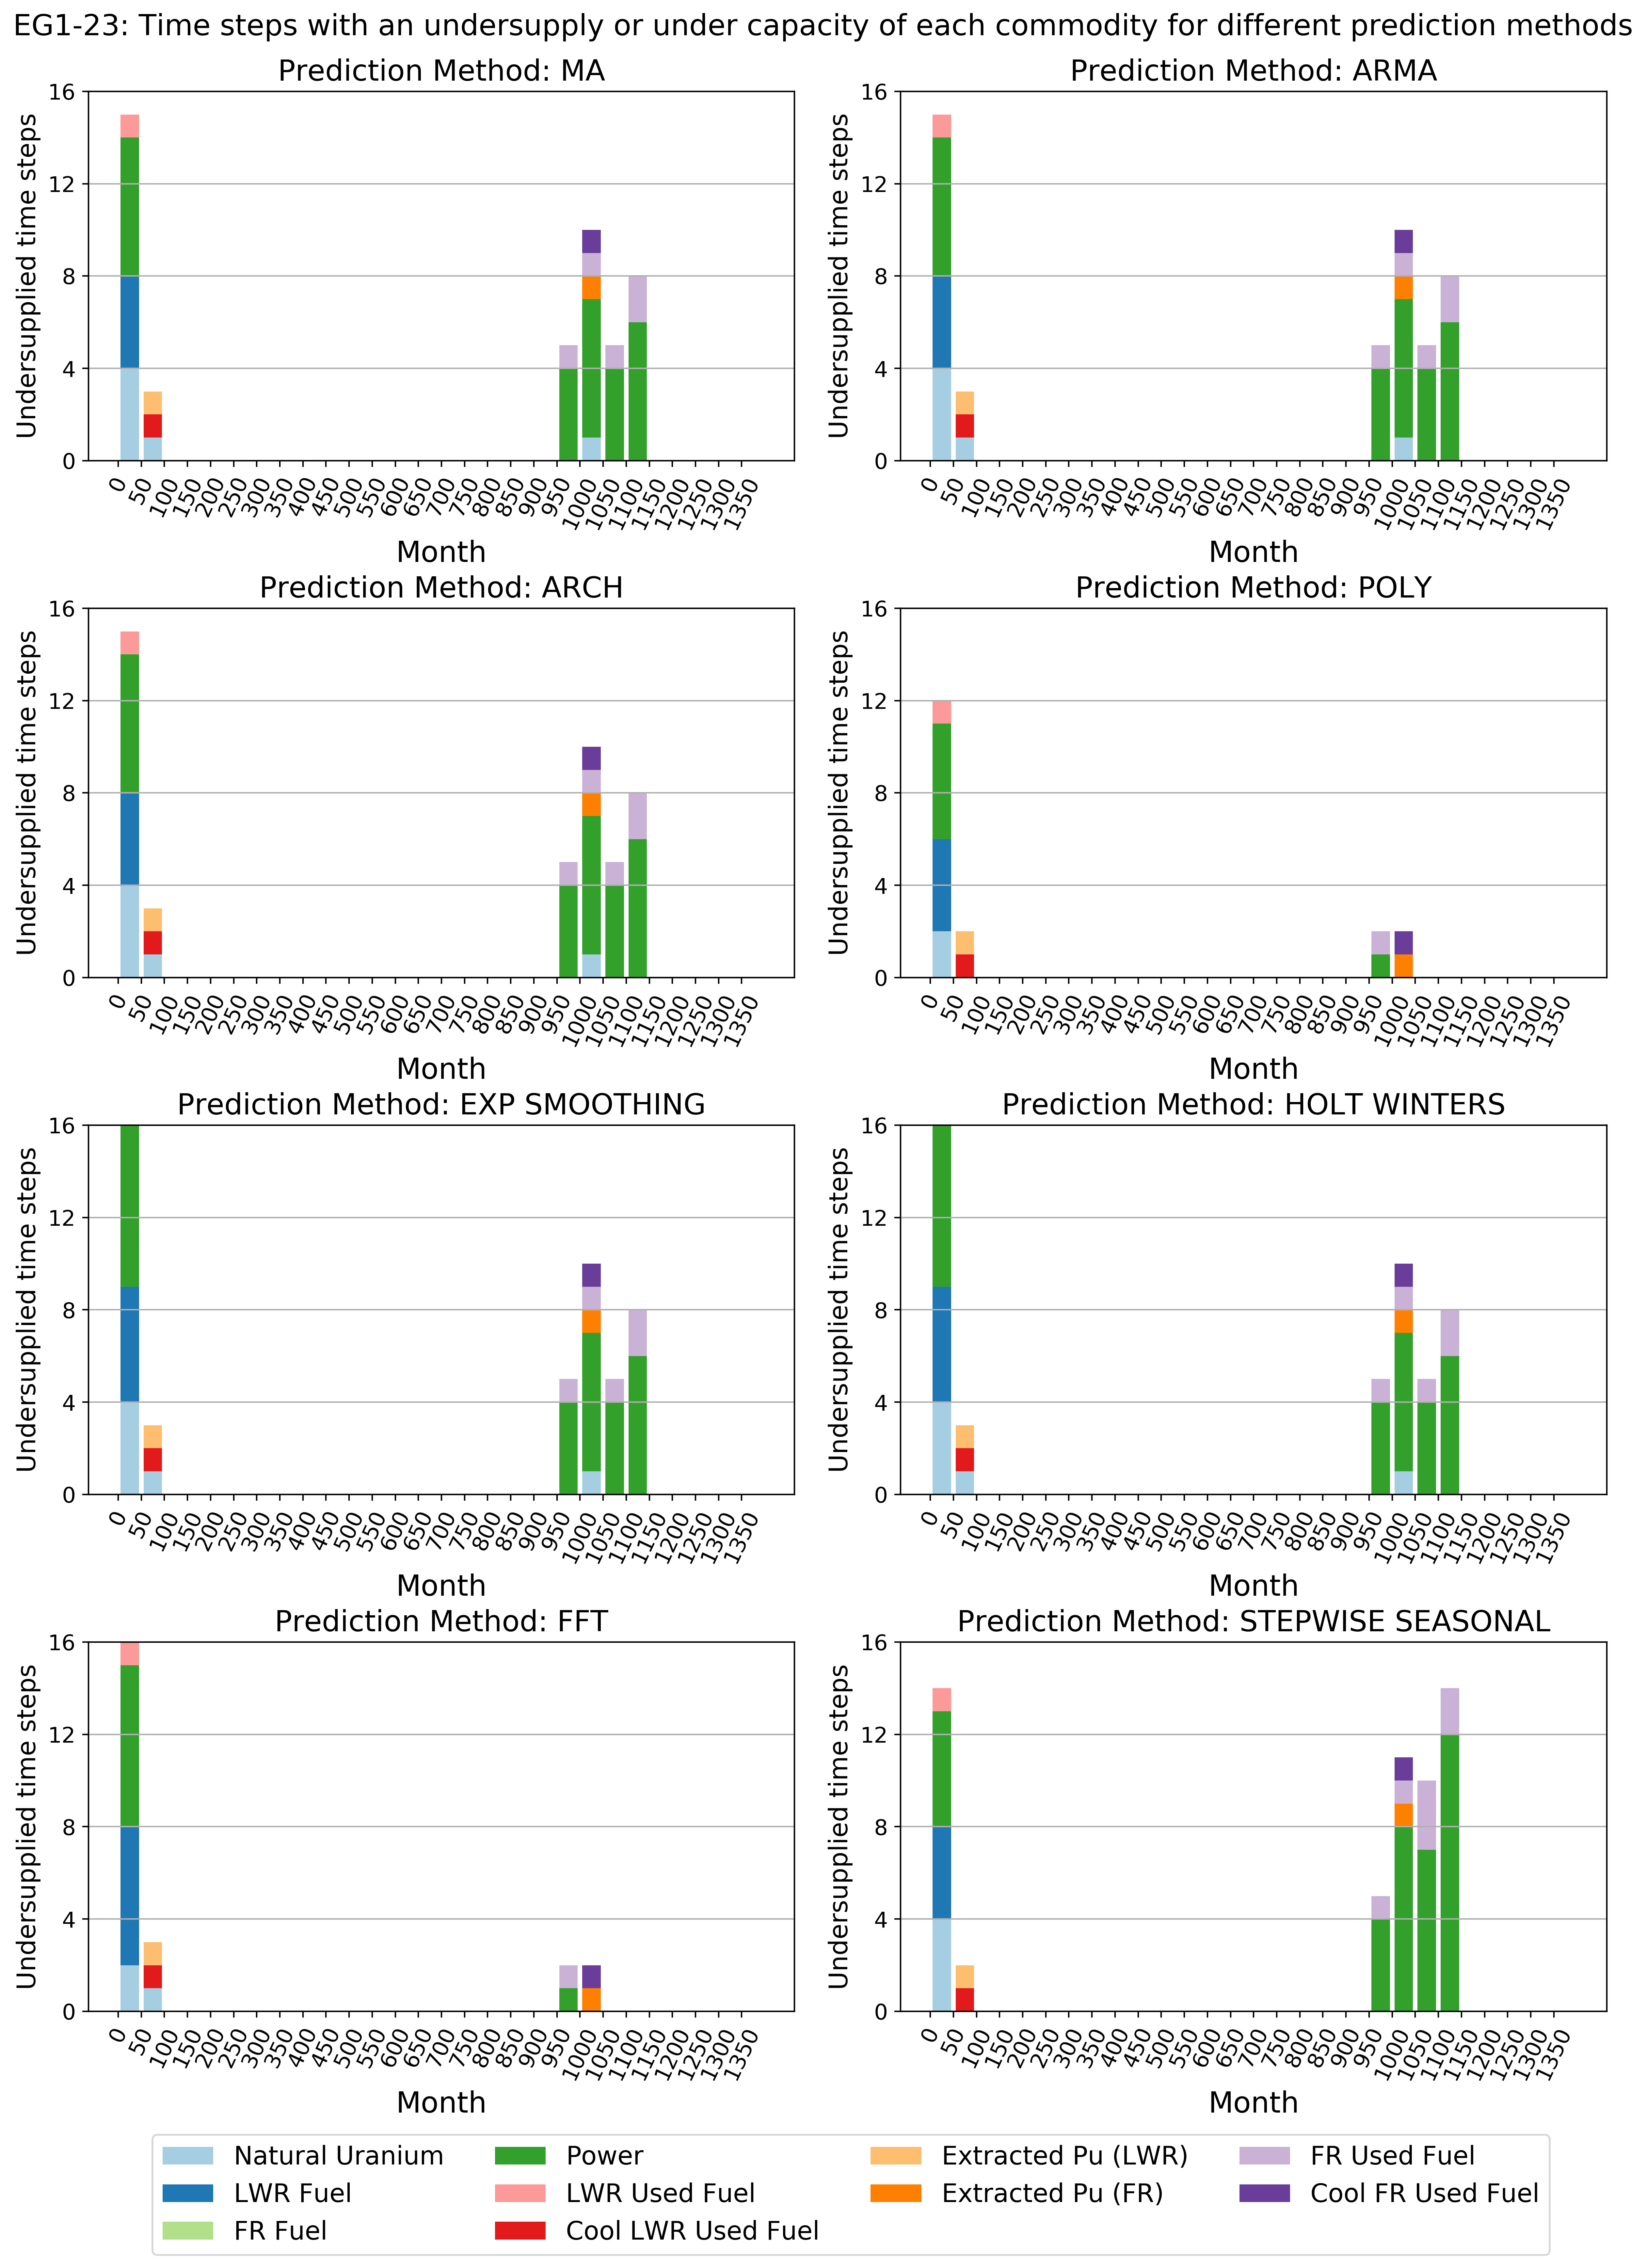
\includegraphics[width=1.2\linewidth]{eg01-23-histogram.png} 
	\caption{
	EG01-23 transition scenario with constant power demand. 
	Each subplot shows the total number of time steps in which there exists 
	undersupply and under capacity of commodities for each prediction method. 
	The different colors represent different commodities, and each time bin 
	refers to a specific time periods in the simulation.
	The \texttt{POLY} method performs the best, with the least number of 
	time steps with undersupply and under capacity.}
	\label{fig:eg23under}
\end{figure}

\begin{figure}[]
	\centering
	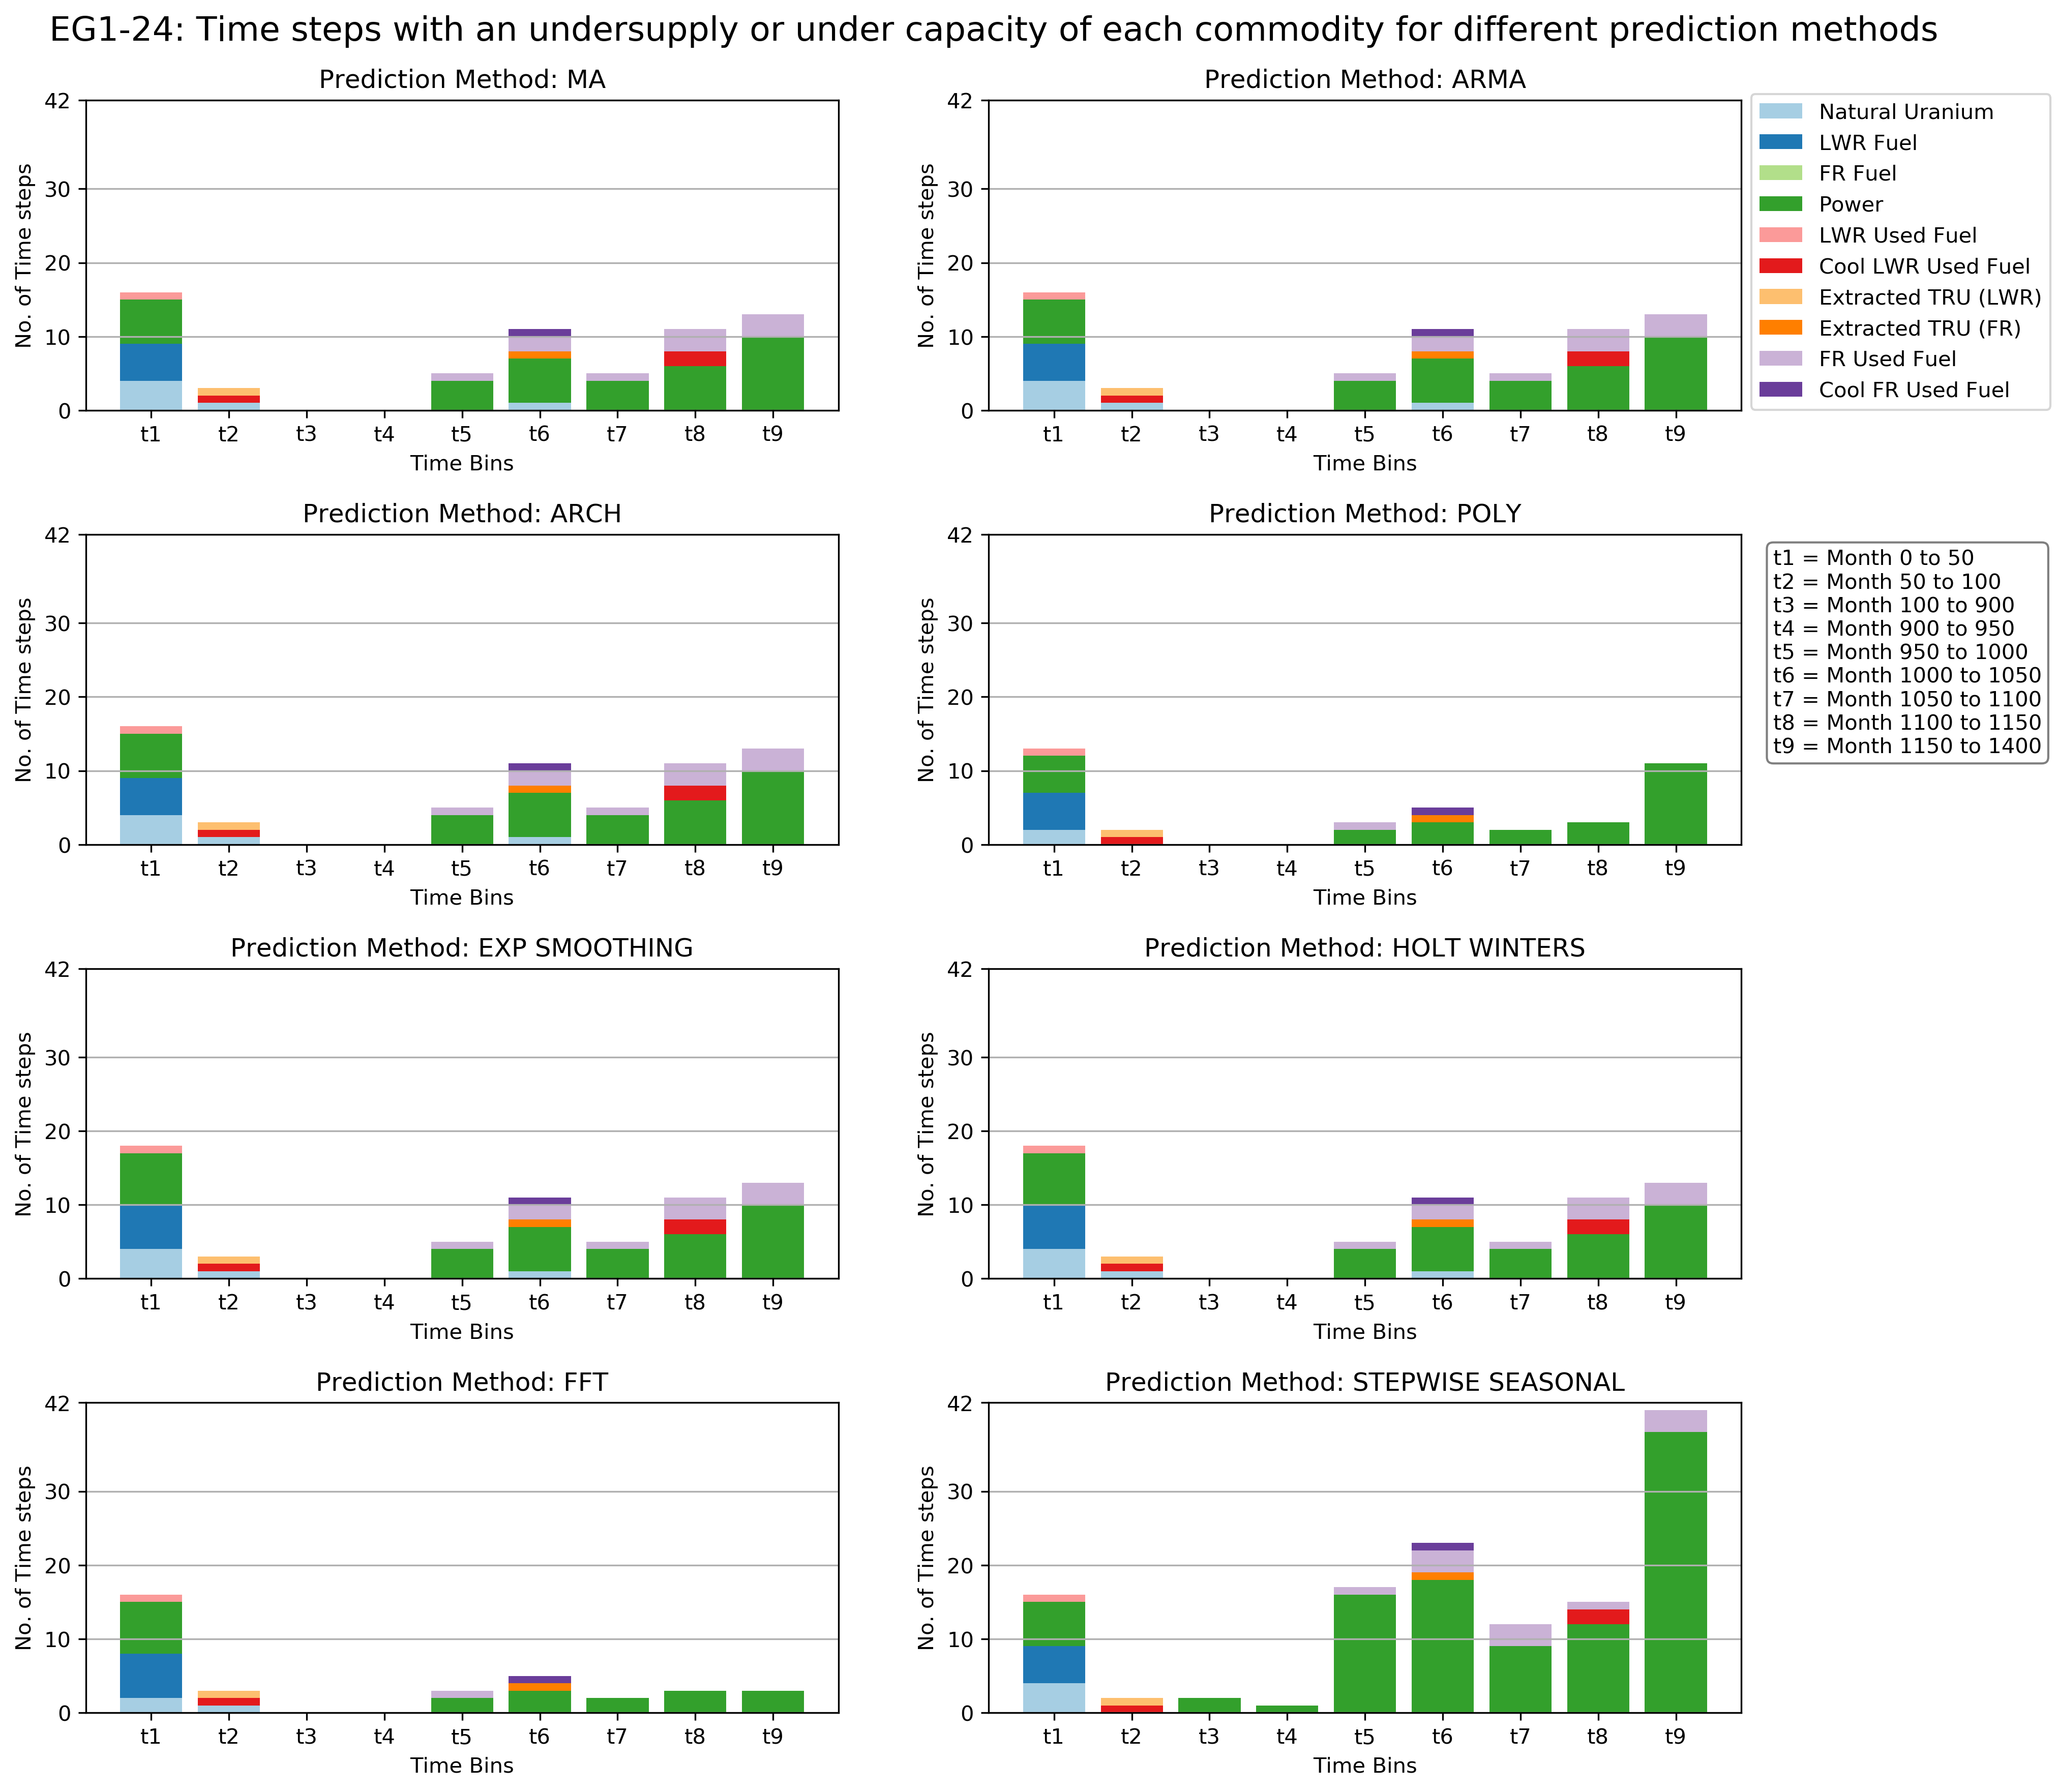
\includegraphics[width=1.2\linewidth]{eg01-24-histogram.png} 
	\caption{
	EG01-24 transition scenario with linearly increasing power demand. 
	Each subplot shows the total number of time steps in which there exists 
	undersupply and under capacity of commodities for each prediction method. 
	The different colors represent different commodities, and each time bin 
	refers to a specific time periods in the simulation.
	The \texttt{FFT} method performs the best, with the least number of 
	time steps with undersupply and under capacity.}
	\label{fig:eg24under}
\end{figure}

\begin{table}[]
	\centering
		\caption{Undersupply and oversupply of power for EG01-EG23,24,29,30 
		transition scenarios for varying prediction methods.}
		\label{tab:all-power}
		\footnotesize
        \begin{tabularx}{\textwidth}{l|RRRR}
		\hline
		& \multicolumn{3}{|c}{\textbf{Power Undersupplied Time Steps}} \\ \hline
		\textbf{Algorithm} & \textbf{EG01-EG23}  & 
		\textbf{EG01-EG24}   & \textbf{EG01-EG29} & 
		\textbf{EG01-EG30} \\ \hline
		\texttt{MA}     		    & 26 	& 36  &  15  & 24 \\ 
		\texttt{ARMA}     	    & 26 	& 36  &  15  & 24\\ 
		\texttt{ARCH}     	    &  26 	& 36  &  15  & 21\\ 
		\texttt{POLY}      		&  6 	& 65  &  4 &  9\\ 
		\texttt{EXP-SMOOTHING} 	& 27 	& 37  & 16 & 25\\ 
		\texttt{HOLT-WINTERS}  	& 27 	& 37  & 16 & 25\\ 
		\texttt{FFT}       		& 8 	& 20  & 5 & 9\\ 
		\texttt{SW-SEASONAL}    & 36 	& 107 & 14 & 51\\ \hline
	\end{tabularx}
\end{table}

From Figures \ref{fig:eg23under}, \ref{fig:eg24under}, and Table 
\ref{tab:all-power}, we can see that the \texttt{POLY} method 
performs best for constant power transition scenarios, 
and the \texttt{FFT} method performs best for linearly increasing 
power transition scenarios. 
Undersupply and under-capacity of commodities occur during two main time periods: 
initial demand for the commodity and during the transition period.
To further \deploy's primary objective of minimizing the power undersupply, 
sensitivity analysis of the power supply buffer is conducted 
with the best-performing prediction method for each transition scenario.  

\subsection{Sensitivity Analysis}
We conducted a sensitivity analysis of the power buffer size for the
EG01-EG23, EG01-24, EG01-29, and EG01-30 transition scenarios. 
Varying the power buffer size does not impact the number of 
undersupply time steps for the EG01-EG23 and EG01-EG29 constant 
power demand transition scenarios with the \texttt{POLY} prediction method.
In Table \ref{tab:all-power}, there are 6 and 4 time steps
in which there is power undersupply for the EG01-EG23 and EG01-29 
transition scenarios, respectively. 
As seen in figure \ref{fig:eg23under}, these undersupply time 
steps occur at the beginning of the simulation and for one 
time step when the transition begins. 
We expected this since without time-series data 
at the beginning of the simulation, \deploy takes a few 
time steps to collect time-series data about power demand 
to predict and start deploying reactor and supporting 
fuel cycle facilities. 
When the transition begins, power is undersupplied for one 
time step, following this, \deploy accounts for the 
undersupply by deploying facilities to meet power demand.
Therefore, we minimized the power undersupply for constant 
power EG01-EG23 and EG01-EG29 transition scenarios with 
a 0MW power supply buffer. 

We varied the power buffer size for the EG01-24 and EG01-30 
linearly increasing power demand transition scenarios. 
Figures \ref{fig:eg24-bufplot}, \ref{fig:eg30-bufplot}, 
and Table \ref{tab:buff_size} 
show that increasing the buffer size decreases the number of 
power undersupply time steps. 
For EG01-24, the cumulative undersupply plateaus at 6000MW, 
and for EG01-30, the cumulative undersupply is smallest 
for a buffer size of 8000MW.
These undersupply time 
steps occur at the beginning of the simulation and for one 
time step when the transition begins. 
We expected this since without time-series data 
at the beginning of the simulation, \deploy takes a few 
time steps to collect time-series data about power demand 
to predict and start deploying reactor and supporting 
fuel cycle facilities. 
Therefore, a buffer of 6000MW and 8000MW minimizes 
the power undersupply for EG01-EG24 and EG01-EG30, respectively.

\begin{figure}[]
	\centering
	\begin{subfigure}[t]{\textwidth}
		\centering
		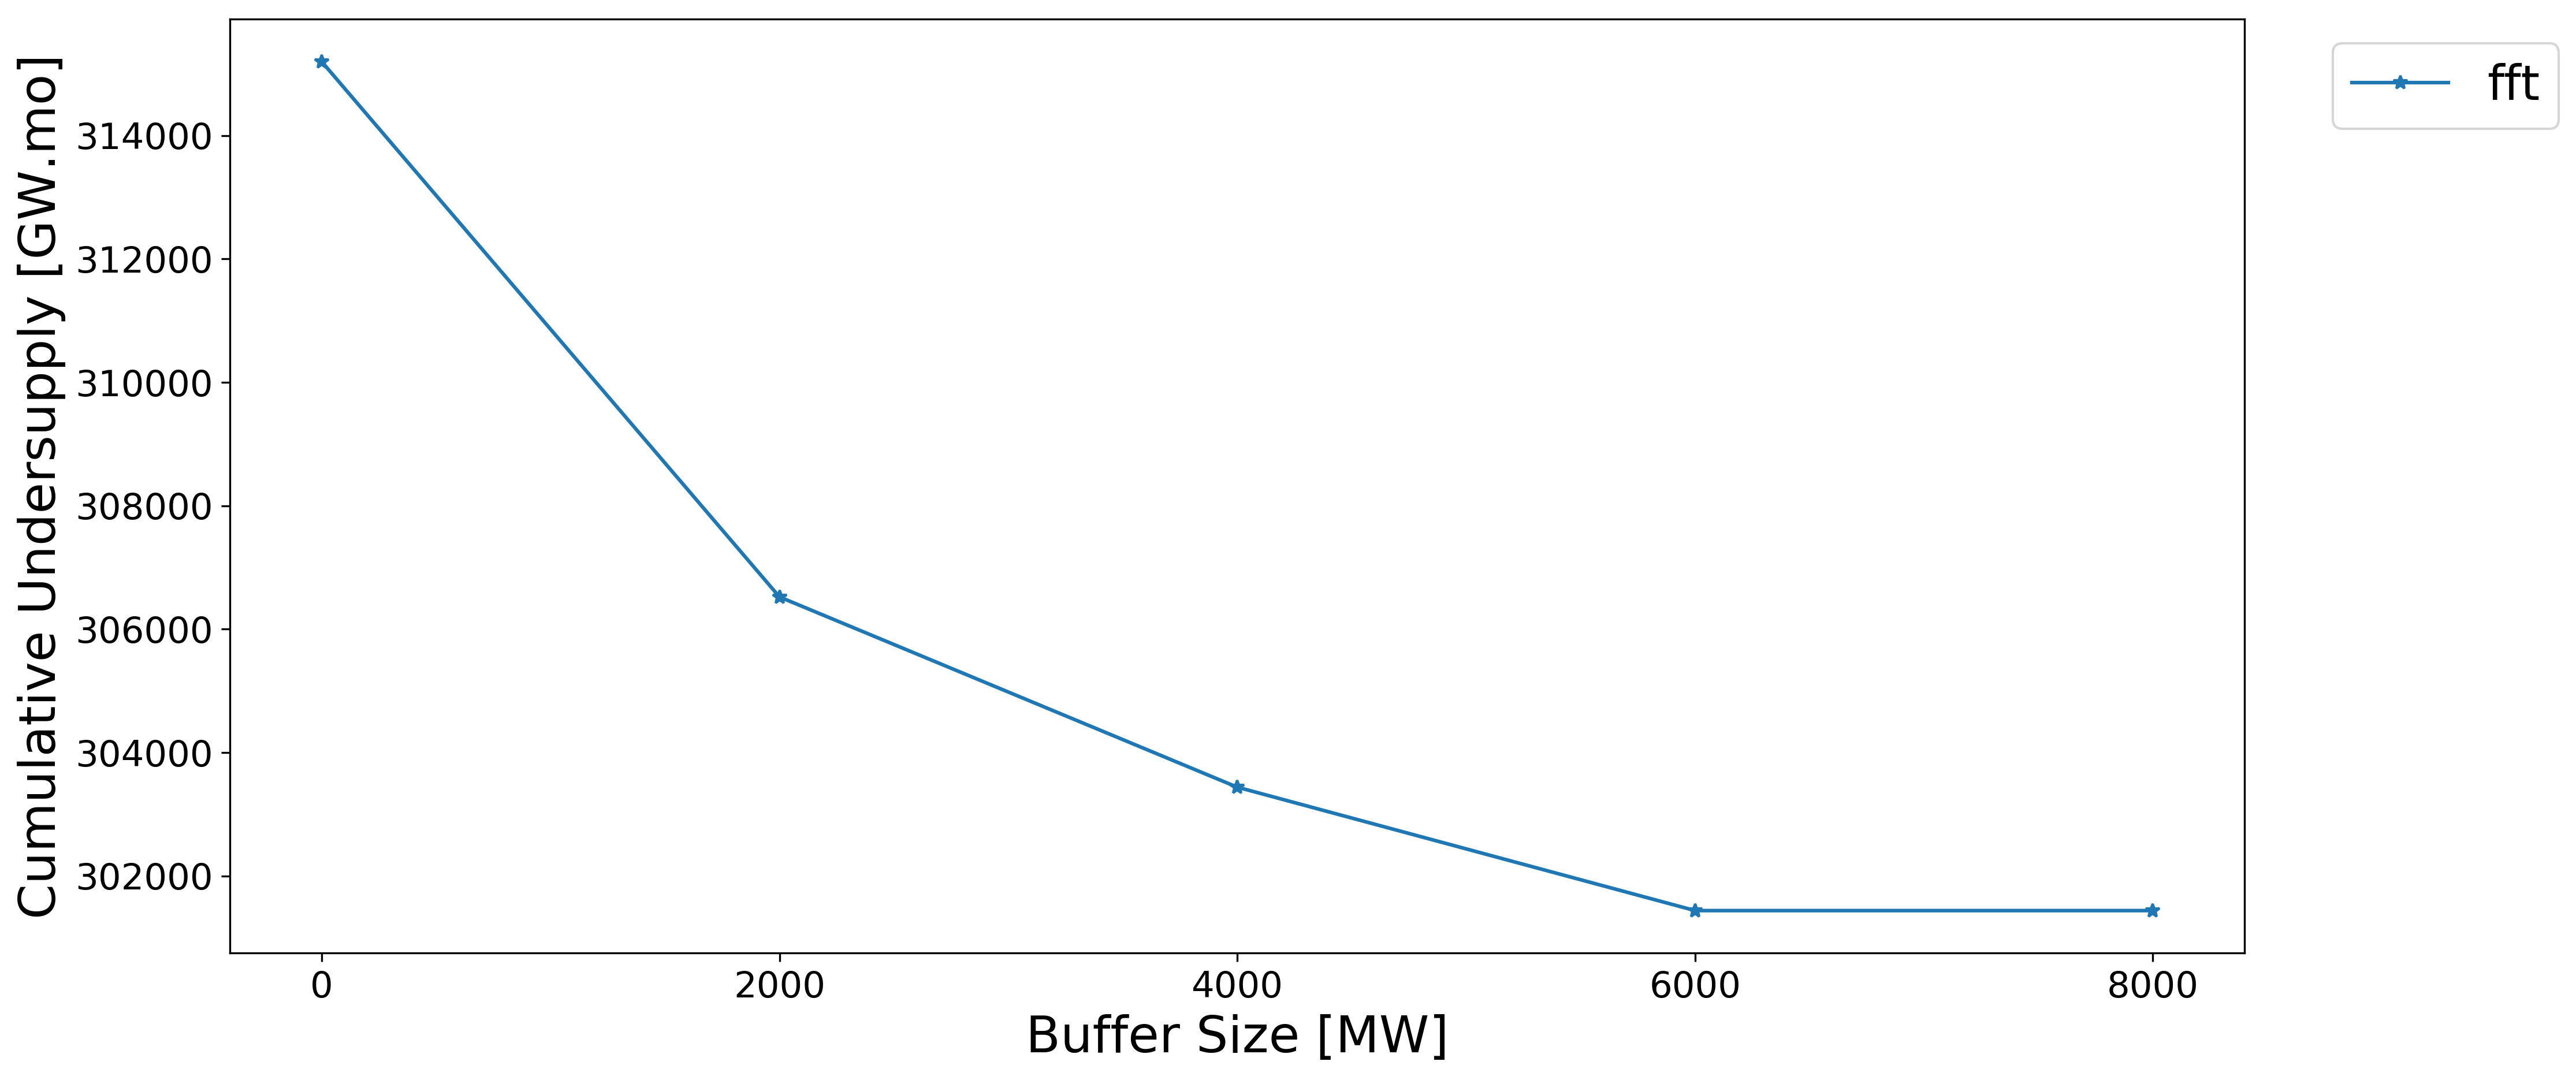
\includegraphics[width=\linewidth]{24-sens-buffer.png} 
		\caption{EG01-24: Power buffer size vs. cumulative undersupply}
		\label{fig:eg24-bufplot}
	\end{subfigure}
	\begin{subfigure}[t]{\textwidth}
		\centering
		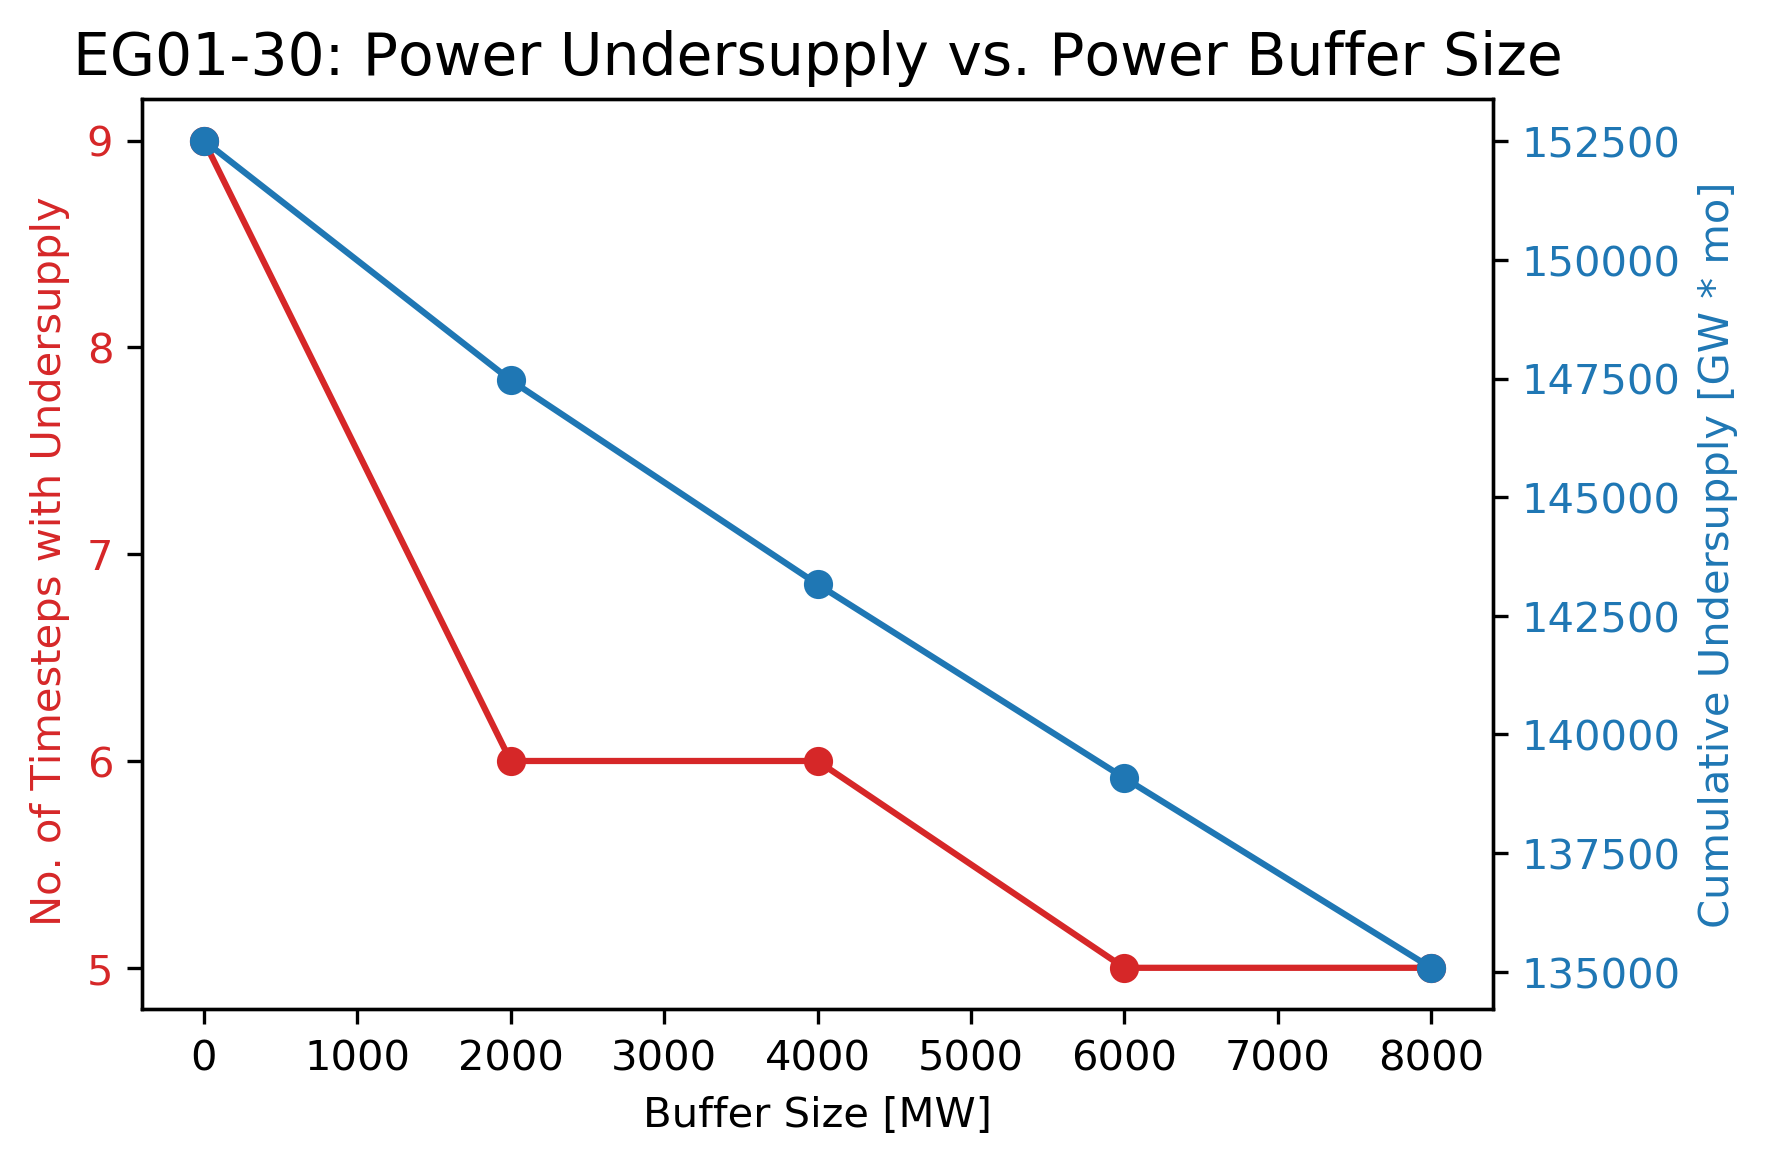
\includegraphics[width=\linewidth]{30-sens-buffer.png} 
		\caption{EG01-30: Power buffer size vs. cumulative undersupply}
		\label{fig:eg30-bufplot}
	\end{subfigure}
	\hfill
	\caption{The effect of sensitivity analysis of power buffer size on cumulative 
	undersupply of power for EG01-EG24 and EG01-EG30 transition scenarios 
	with linearly increasing power demand using the \texttt{FFT} prediction method.}
	\label{fig:sabuffer}
\end{figure}

\begin{table}[]
	\centering
	\caption{The effect of sensitivity analysis of power buffer size on cumulative 
	undersupply of power for EG01-EG24 and EG01-EG30 transition scenarios with linearly 
	increasing power demand using the \texttt{FFT} prediction method.}
	\label{tab:buff_size}
	\footnotesize
		\begin{tabular}{r|lrr}
                \hline
        \textbf{Buffer [MW]}     & \textbf{Undersupply}             & \textbf{EG01-24}   & \textbf{EG01-30} \\
		\hline
		\textbf{0}             & Time steps $[\#]$ & 20 & 9\\  
                      & Energy $[GW\cdot mo]$    & 315791 & 152517 \\ \hline
		\textbf{2000}          & Undersupplied $[\#]$ & 9 & 6 \\  
        	      & Energy $[GW\cdot mo]$    & 306520 & 147166 \\ \hline
        \textbf{4000}          & Time steps $[\#]$ & 8 & 6 \\  
				  & Energy $[GW\cdot mo]$    & 303438 & 143166 \\ \hline
		\textbf{6000}          & Time steps $[\#]$ & 7 & 5 \\  
		& Cumulative $[GW]$    & 303438 & 139083 \\ \hline
        \textbf{8000}          & Time steps $[\#]$ & 7 & 5  \\  
	              & Energy $[GW\cdot mo]$    & 303438 & 135083 \\ \hline
	\end{tabular}
\end{table}

\subsection{Best Performance Models}
Table \ref{tab:bestinputs} shows the \deploy input parameters for
EG01-EG23, EG01-EG24, EG01-EG29, and EG01-EG30 transition scenarios
that minimize the undersupply of power and 
undersupply and under-capacity of the other commodities
in the simulation. 
The need for commodity supply buffers is a reflection of reality
in which a supply buffer is usually maintained to ensure 
continuity in the event of an unexpected failure in the supply chain.

Figures \ref{fig:23stack} and \ref{fig:30stack} show
time-dependent deployment of reactor and supporting facilities for 
the EG01-23 constant power demand and EG01-30 linearly increasing power demand 
transition scenarios, respectively. 
\deploy automatically deploys reactor and supporting facilities 
to set up a supply chain to meet power demand
during a transition from \glspl{LWR} to \glspl{SFR} for EG01-23, 
and from \glspl{LWR} to \gls{MOX} \glspl{LWR} and \glspl{SFR} for 
EG01-30. 
EG01-24 and EG01-29 facility deployment plots are similar to 
EG01-23 and EG01-30, respectively, therefore they are not shown. 

\begin{table}[]
	\centering
	\begin{tabular}{r|cccc}
	\hline
	\multicolumn{1}{c|}{\multirow{2}{*}{\textbf{Input Parameter}}} & \multicolumn{4}{c}{\textbf{Simulation Description}}                                                                                                                                                                                                                                                       \\ \cline{2-5}
	\multicolumn{1}{c|}{}                                          & \multicolumn{1}{l}{\textbf{EG01-23}}                                                                 & \textbf{EG01-24}                  & \textbf{EG01-29}                 &\textbf{EG01-30}                                                  \\ \hline
	\textbf{Demand Driving}                                      & Power & Power & Power & Power                                                                                                                                                                                                                                                                                \\ 
	\textbf{Commodity} \\ \hline  
	\textbf{Demand}                                               & 60000                                                                                & 60000 & 60000                     &  60000                                        \\ 
	\textbf{Equation [MW]} & &$+250t/12$& &$+250t/12$ \\ \hline 
	\textbf{Prediction}                                             & \texttt{POLY}       & \texttt{FFT}             & \texttt{POLY}         &  \texttt{FFT}    \\ 
	\textbf{Method} \\ \hline 
	\textbf{Deployment}   & Installed & Installed  & Installed   & Installed    \\                                                                                                                                                                                 
	\textbf{Driving Method} & Capacity & Capacity  & Capacity   & Capacity \\ \hline 
	\textbf{Fleet Share} &  MOX: 85\% &  MOX: 85\% &  MOX: 85\% &  MOX :85\%     \\
	\textbf{Percentage} &SFR: 15\%&SFR: 15\%&SFR: 15\%&SFR: 15\%\\ \hline
	\textbf{Buffer type}                                                    & \multicolumn{4}{c}{Absolute}                                                                                                                                                                                                                                                               \\ \hline
	\textbf{Power Buffer}                                                  & 0 & 6000 & 0 & 8000 \\ 
	\textbf{Size [MW]} \\ \hline \end{tabular}
	\caption{\deploy's input parameters for EG01-EG23, EG01-EG24, EG01-EG29, and 
	EG01-EG30 transition scenarios
	that minimizes undersupply of power and minimizes 
	the undersupply and under-capacity of the other facilities. }
	\label{tab:bestinputs}
	\end{table}

\begin{figure}[]
	\centering
	\begin{subfigure}[t]{1.2\textwidth}
		\centering
		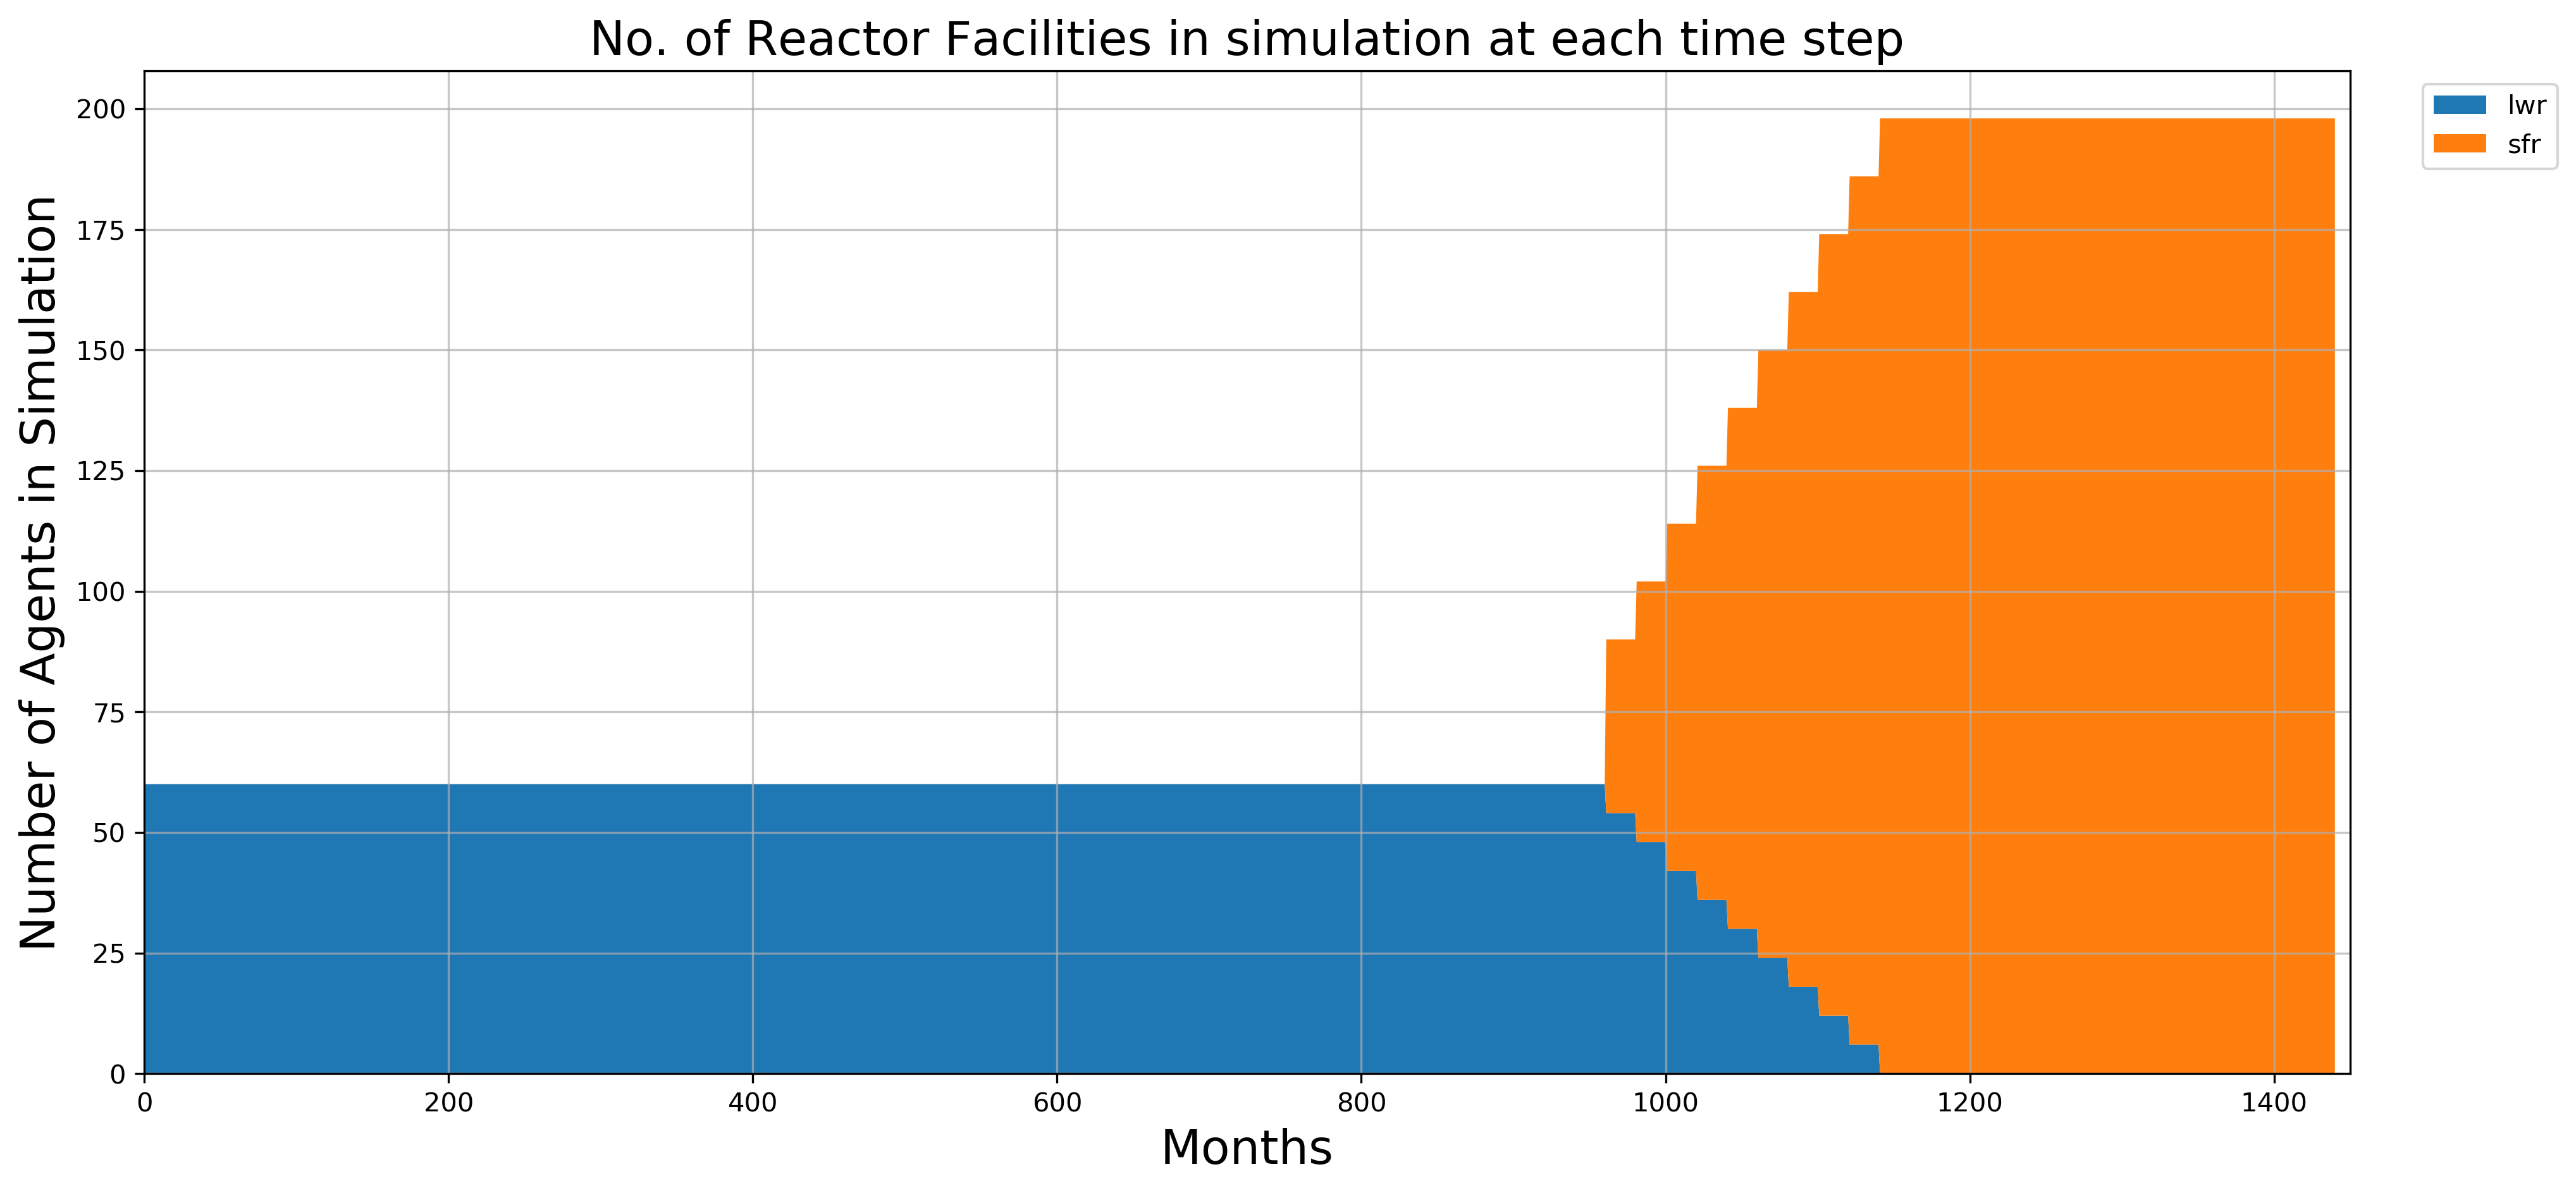
\includegraphics[width=\linewidth]{eg23-stack_reactor.png} 
		\caption{EG01-23: Reactor Deployment}
		\label{fig:23reactor}
	\end{subfigure}
	\vspace{1cm}
	\begin{subfigure}[t]{1.2\textwidth}
		\centering
		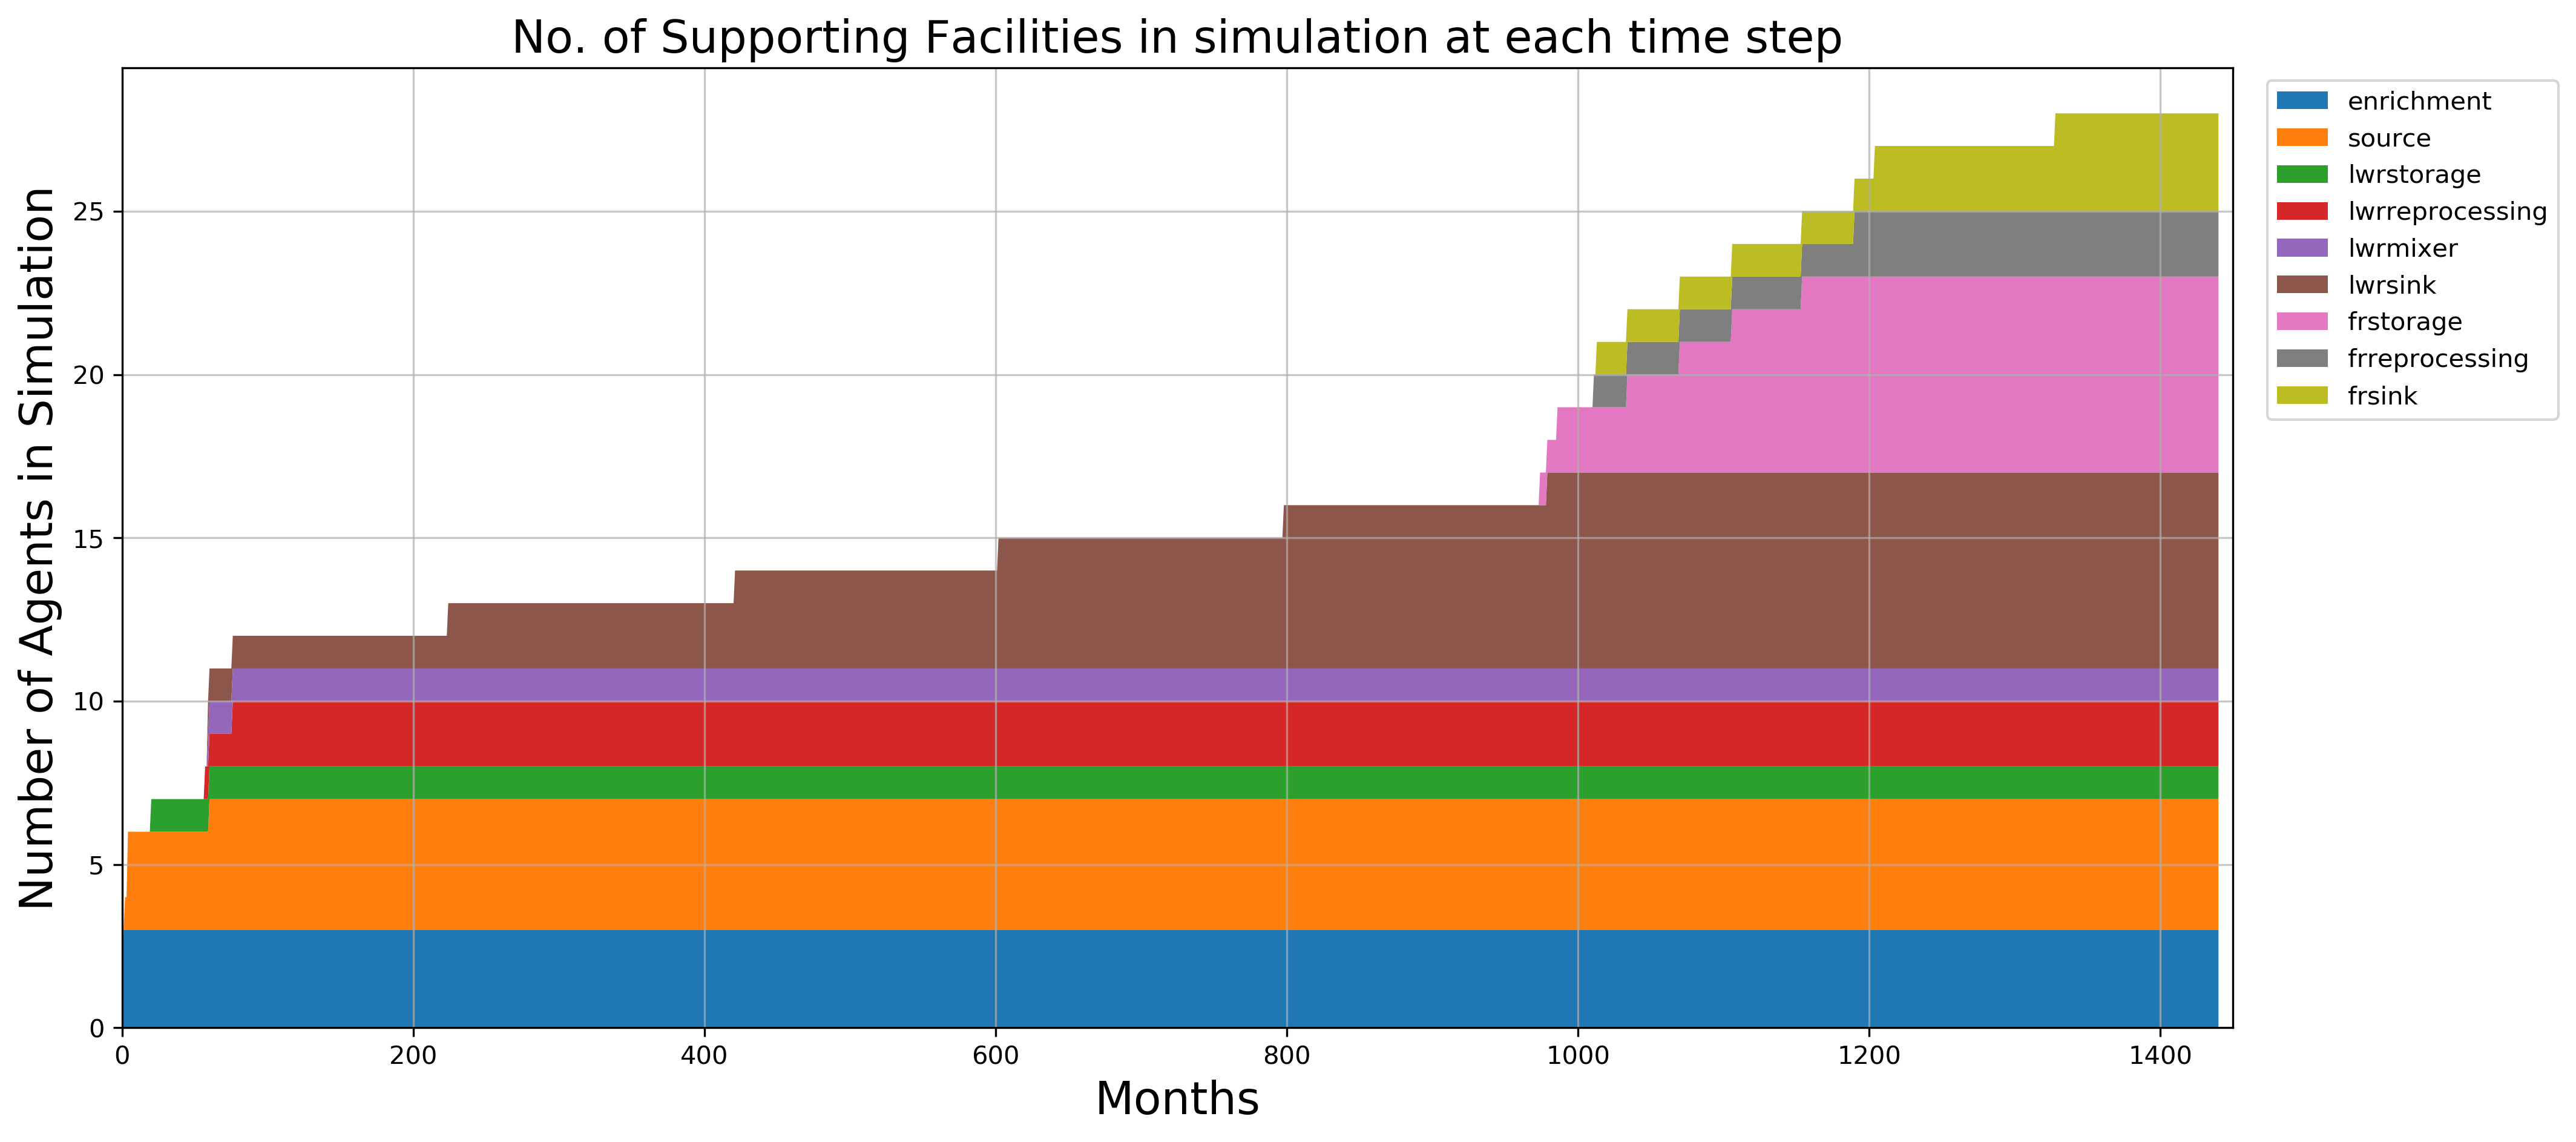
\includegraphics[width=\linewidth]{eg23-stack_support.png} 
		\caption{EG01-23: Supporting Facility Deployment}
		\label{fig:23support}
	\end{subfigure}
	\hfill
	\caption{Time dependent deployment of reactor and supporting facilities in 
	the EG01-23 constant power demand transition scenario. 
	\deploy automatically deploys reactor and supporting facilities 
	to setup a supply chain to meet constant power demand of $60000$ MW
	during a transition from \glspl{LWR} to \glspl{SFR}. }
	\label{fig:23stack}
\end{figure}

\begin{figure}[]
	\centering
	\begin{subfigure}[t]{1.2\textwidth}
		\centering
		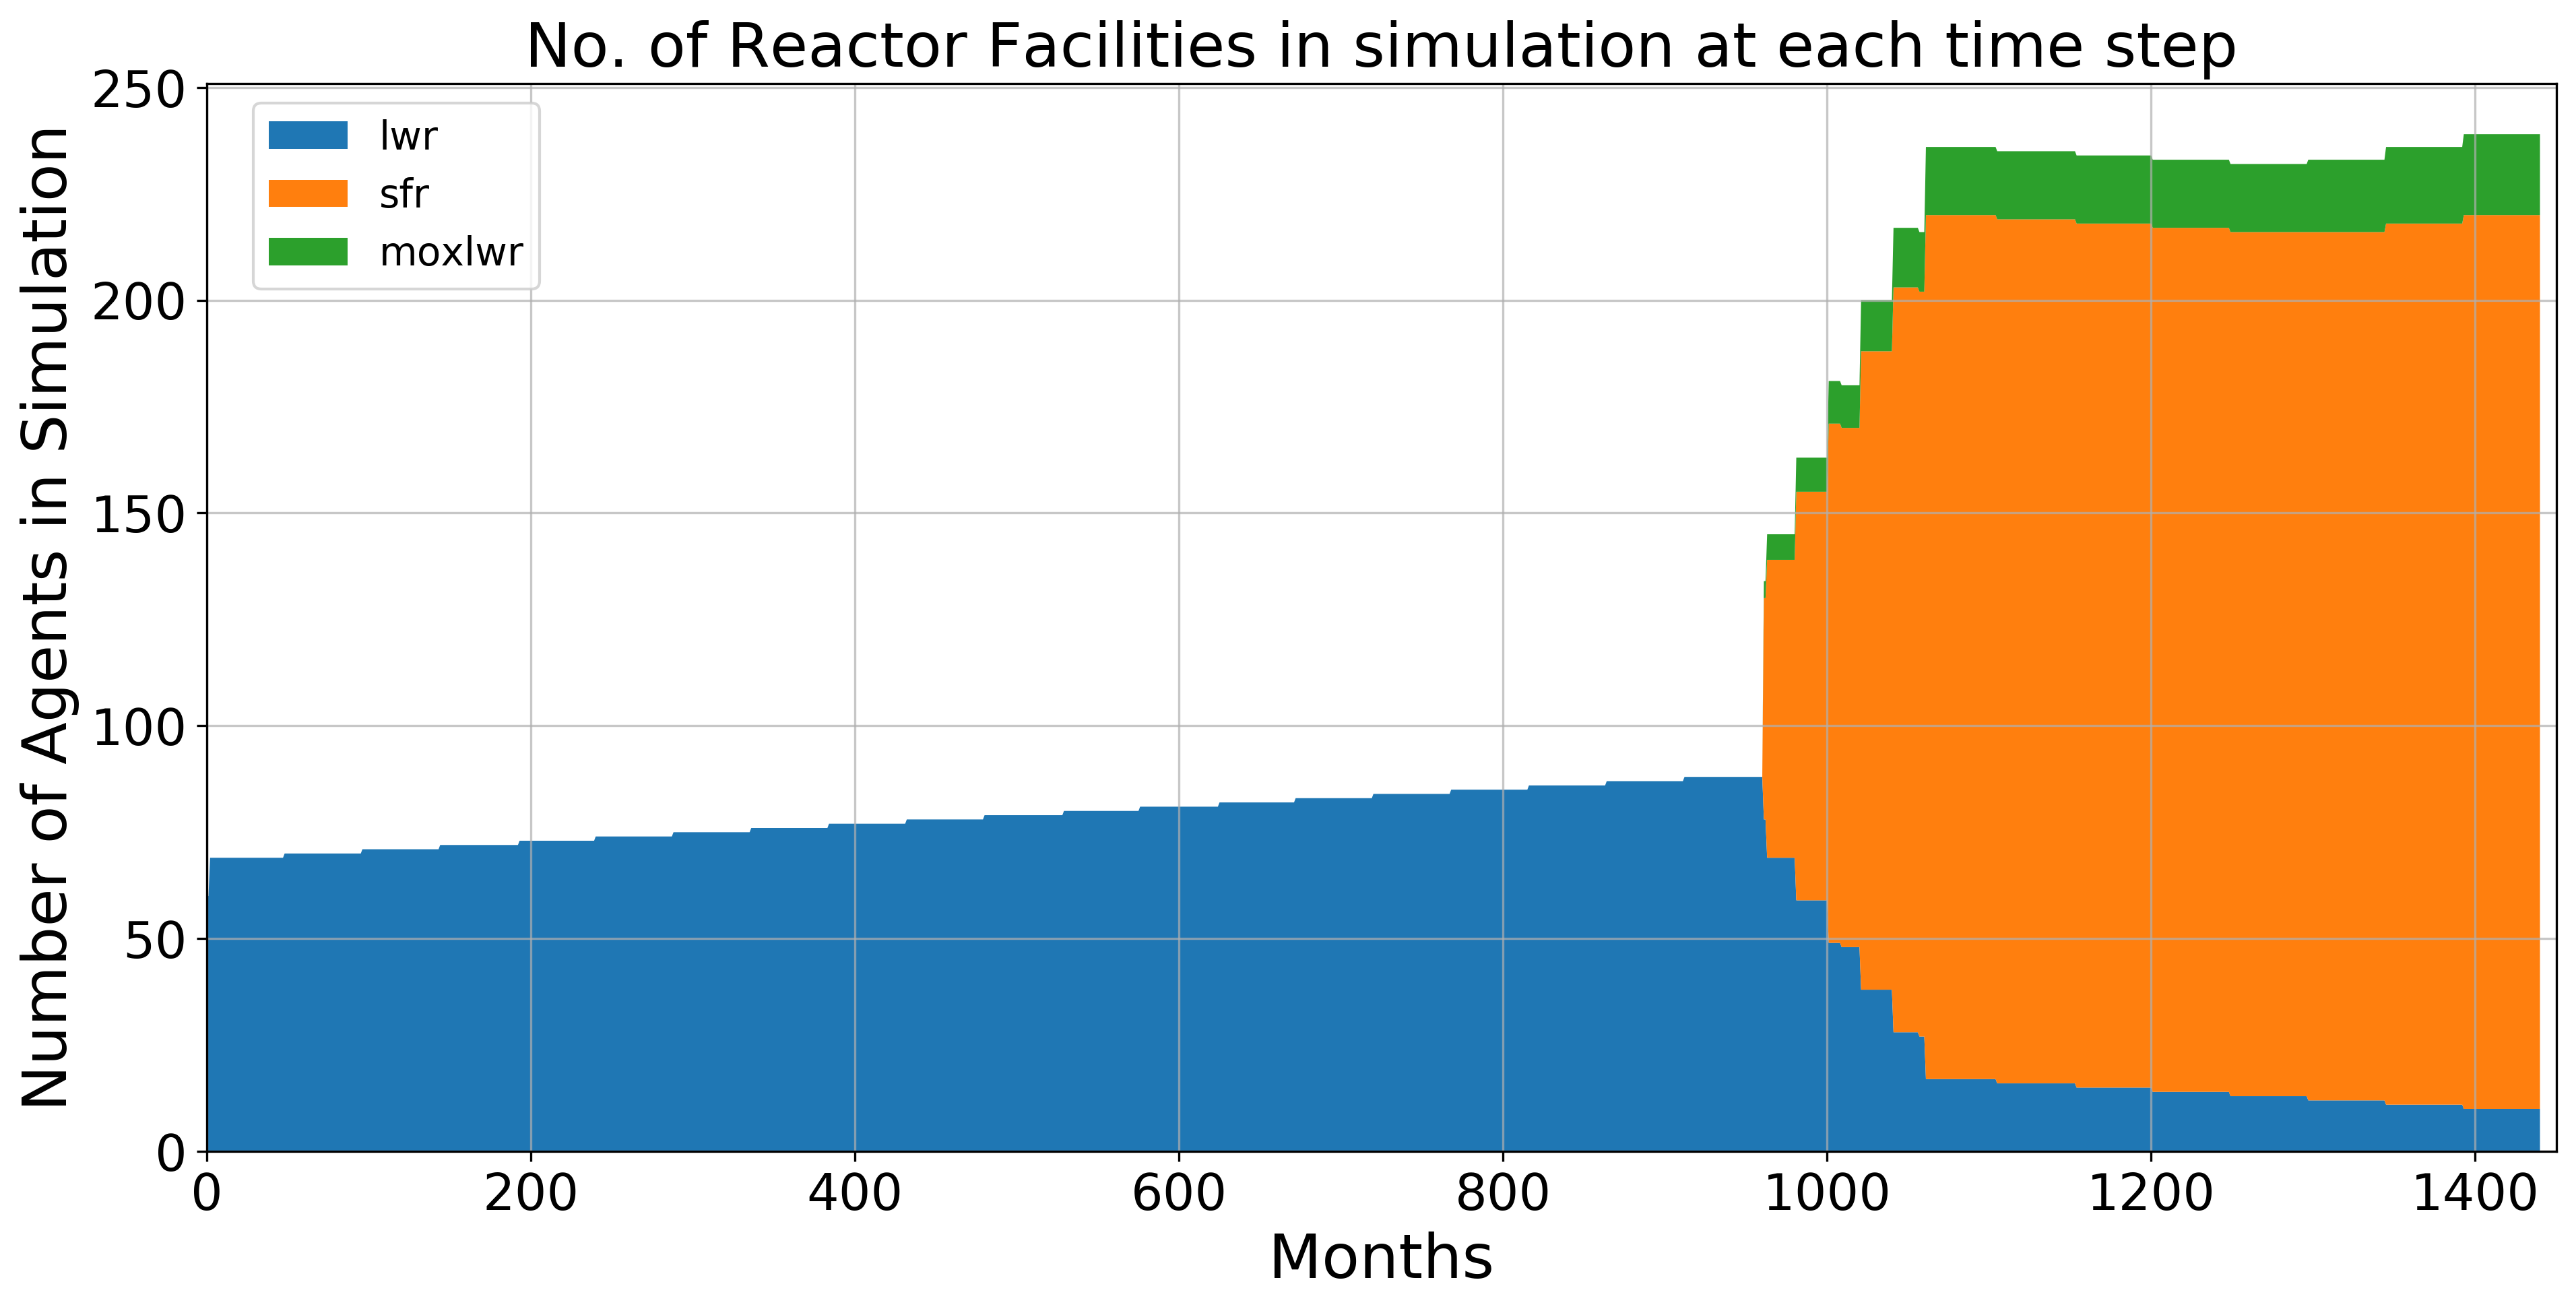
\includegraphics[width=\linewidth]{eg30-stack_reactor.png} 
		\caption{EG01-30: Reactor Deployment}
		\label{fig:30reactor}
	\end{subfigure}
	\vspace{1cm}
	\begin{subfigure}[t]{1.2\textwidth}
		\centering
		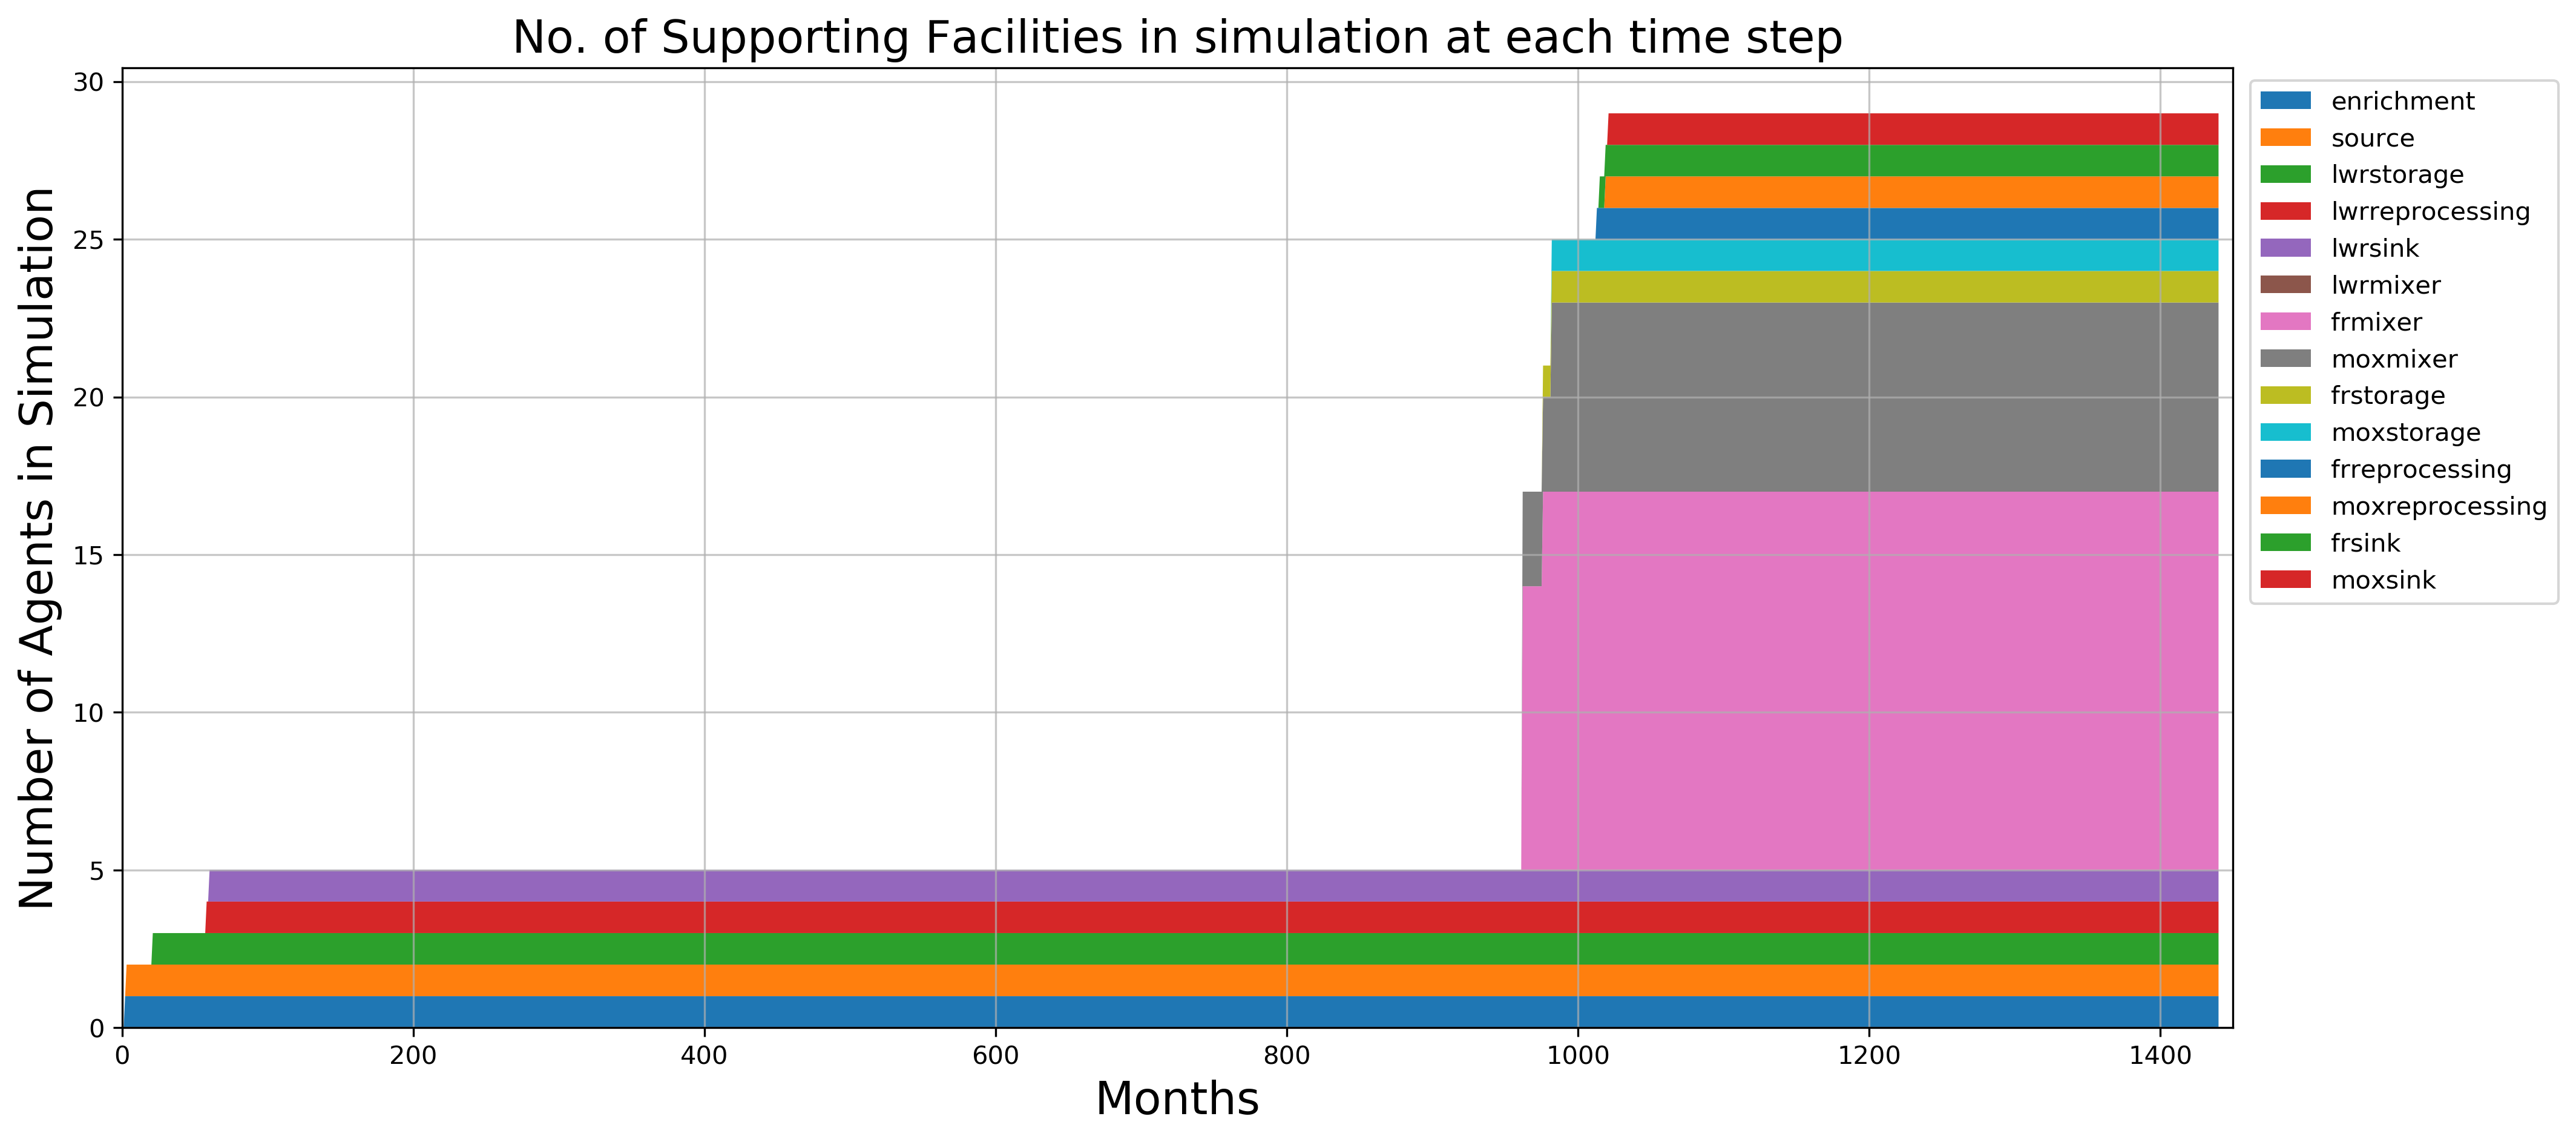
\includegraphics[width=\linewidth]{eg30-stack_support.png} 
		\caption{EG01-30: Supporting Facility Deployment}
		\label{fig:30support}
	\end{subfigure}
	\hfill
	\caption{Time dependent deployment of reactor and supporting facilities in 
	the EG01-30 linearly increasing power demand transition scenario. 
	\deploy automatically deploys reactor and supporting facilities 
	to setup a supply chain to meet linearly increasing power demand of $60000 + 250t/12$ MW
	during a transition from \glspl{LWR} to MOX LWRs and \glspl{SFR}. }
	\label{fig:30stack}
\end{figure}

\begin{table}[]
	\centering
        \caption{Undersupply/capacity of key commodities for the best performing EG01-EG23,24,29,30 transition scenarios.}
		\label{tab:all-power}
		\footnotesize
        \begin{tabular}{lcccc}
		\hline
		& \multicolumn{3}{c}{\textbf{No. of Time Steps with Undersupply}} \\ \hline
		\textbf{Transition Scenario} & EG01-EG23 & 
		EG01-EG24 & EG01-EG29 & EG01-EG30 \\ \hline 
		\textbf{Commodities} \\ 
		Natural Uranium		    & 2 	& 3  &  1  & 1 \\ 
		\gls{LWR} Fuel     	    & 4 	& 6  &  1  & 2\\ 
		\gls{SFR} Fuel     	    &  0 	& 0  &  2  & 2\\ 
		\gls{MOX} \gls{LWR} Fuel &-&-&2&2 \\
		Power      				&  6 	& 7  &  4 &  5\\ 
		\gls{LWR} Spent Fuel	& 1 	& 1  & 1 & 1\\ 
		\gls{SFR} Spent Fuel     	    &  1 	& 1  &  1  & 1\\ 
		\gls{MOX} \gls{LWR} Spent Fuel &-&-&1&1 \\ \hline 
	\end{tabular}
\end{table}

% demonstration of d3ploy's capabilities (basic transition cases) 
% comparison of prediction methods
% - Tables: table 10 from report + more buffer size steps, 
% - Example model   
\FloatBarrier
\section{Conclusion}
In this paper, we demonstrate 

By carefully selecting \deploy parameters, we are able to 
effectively automate setting up of transition scenarios for 
different evaluation groups. 
This is more efficient than the previous efforts that
required a user to manually calculate and use trial and error 
to set up the deployment scheme for the supporting fuel cycle 
facilities. 
Transition scenario simulations set up this way are sensitive 
to changes in the input parameters. 
This becomes an arduous process since a slight change in one 
of the input parameters would result in the need to recalculate 
the deployment scheme.  
Therefore, by automating this process, the user can vary input parameters 
in the simulation and \deploy will automatically adjust the
deployment scheme to meet the new constraints. 
\FloatBarrier
\section{Future Work}
A sensitivity analysis varying the prediction method for 
each commodity in each simulation could be conducted. 
Since each commodity has a different pattern of demand and 
supply, the prediction method that best matches a specific 
commodity can be determined. 
\FloatBarrier
\section{Acknowledgments}
\gls{DOE} Office of Nuclear Energy funds this research through 
the  Nuclear Energy University Program (Project 16-10512, DE-NE0008567) 
`Demand-Driven Cycamore Archetypes'. The authors want to thank 
members of the \gls{ARFC} group at the University of Illinois at 
Urbana-Champaign. 
Special thanks to Kip Kleimenhagen and Matthew Kozak 
for their excellent proofreading help. 
We also thank our colleagues from the \Cyclus community
for collaborative \Cyclus development.

The authors contributed to this work as described below. 
Gwendolyn J. Chee conceived and designed the simulations, wrote the paper, 
prepared figures and/or tables, performed the computation work, contributed to
and validated the software product, and reviewed drafts of the paper. 
Roberto E. Fairhurst Agosta performed the computation work and contributed to
the software product. 
Jin Whan Bae conceived and designed the simulations and contributed to and validated
the software product. 
Robert R. Flanagan conceived and designed the simulations and contributed to 
the software product. 
Anthony M. Scopatz conceived and designed the simulations and acquired funding 
support for the project. 
Kathryn D. Huff directed and supervised the work, acquired funding 
support for the project, conceived and designed the simulations, contributed to 
the software product, and reviewed drafts of the paper.
\FloatBarrier

%\nocite{robertson_conceptual_1971} % placeholder until citations appear
\bibliography{2019-ddca}

%%% Random thoughts 
% deploy vs Deploy?

\end{document}
